% !TeX encoding = UTF-8
% !TeX program = xelatex
% !TeX spellcheck = en_US

\documentclass[degree=bachelor]{thuthesis}
  % 学位 degree:
  %   doctor | master | bachelor | postdoc
  % 学位类型 degree-type:
  %   academic(默认)| professional


% 论文基本配置,加载宏包等全局配置
% !TeX root = ../main.tex

% 论文基本信息配置

\thusetup{
  %******************************
  % 注意:
  %   1. 配置里面不要出现空行
  %   2. 不需要的配置信息可以删除
  %******************************
  %
  % 标题
  %   可使用“\\”命令手动控制换行
  %
  title  = {视觉推理},
  title* = {Visual Reasoning},
  %
  % 学位
  %   1. 学术型
  %      - 中文
  %        需注明所属的学科门类,例如:
  %        哲学、经济学、法学、教育学、文学、历史学、理学、工学、农学、医学、
  %        军事学、管理学、艺术学
  %      - 英文
  %        博士:Doctor of Philosophy
  %        硕士:
  %          哲学、文学、历史学、法学、教育学、艺术学门类,公共管理学科
  %          填写“Master of Arts“,其它填写“Master of Science”
  %   2. 专业型
  %      直接填写专业学位的名称,例如:
  %      教育博士、工程硕士等
  %      Doctor of Education, Master of Engineering
  %   3. 本科生不需要填写
  %
  degree-name  = {},
  degree-name* = {},
  %
  % 培养单位
  %   填写所属院系的全名
  %
  department = {自动化系},
  %
  % 学科
  %   1. 学术型学位
  %      获得一级学科授权的学科填写一级学科名称,其他填写二级学科名称
  %   2. 工程硕士
  %      工程领域名称
  %   3. 其他专业型学位
  %      不填写此项
  %   4. 本科生不需要填写
  %
  discipline  = {},
  discipline* = {},
  %
  % 姓名
  %
  author  = {赵文亮},
  author* = {Zhao Wenliang},
  %
  % 指导教师
  %   中文姓名和职称之间以英文逗号“,”分开,下同
  %
  supervisor  = {周杰,教授},
  supervisor* = {Professor Zhou Jie},
  %
  % 副指导教师
  %
  associate-supervisor  = {鲁继文,教授},
  associate-supervisor* = {Professor Lu Jiwen},
  %
  % 联合指导教师
  %
  % joint-supervisor  = {某某某教授},
  % joint-supervisor* = {Professor Mou Moumou},
  %
  % 日期
  %   使用 ISO 格式;默认为当前时间
  %
  % date = {2019-07-07},
  %
  % 密级和年限
  %   秘密, 机密, 绝密
  %
  % secret-level = {秘密},
  % secret-year  = {10},
  %
  % 博士后专有部分
  %
  % clc                = {分类号},
  % udc                = {UDC},
  % id                 = {编号},
  % discipline-level-1 = {计算机科学与技术},  % 流动站(一级学科)名称
  % discipline-level-2 = {系统结构},          % 专业(二级学科)名称
  % start-date         = {2011-07-01},        % 研究工作起始时间
}

%% Put any packages you would like to use here

% 表格中支持跨行
\usepackage{multirow}

\usepackage{subcaption}

% 跨页表格
\usepackage{longtable}

% 固定宽度的表格
\usepackage{tabularx}

% 最全的表格宏包
\usepackage{tabu}

% 表格中的反斜线
\usepackage{diagbox}

% 确定浮动对象的位置,可以使用 H,强制将浮动对象放到这里(可能效果很差)
\usepackage{float}

% 浮动图形控制宏包。
% 允许上一个 section 的浮动图形出现在下一个 section 的开始部分
% 该宏包提供处理浮动对象的 \FloatBarrier 命令,使所有未处
% 理的浮动图形立即被处理。这三个宏包仅供参考,未必使用:
% \usepackage[below]{placeins}
% \usepackage{floatflt} % 图文混排用宏包
% \usepackage{rotating} % 图形和表格的控制旋转

% 定理类环境宏包
\usepackage[amsmath,thmmarks,hyperref]{ntheorem}

\usepackage{mathtools}
% 给自定义的宏后面自动加空白
% \usepackage{xspace}

\usepackage{pifont}% http://ctan.org/pkg/pifont
% keyboard
\usepackage{menukeys}

% 借用 ltxdoc 里面的几个命令。
\def\cmd#1{\cs{\expandafter\cmd@to@cs\string#1}}
\def\cmd@to@cs#1#2{\char\number`#2\relax}
\DeclareRobustCommand\cs[1]{\texttt{\char`\\#1}}

\newcommand*{\meta}[1]{{%
  \ensuremath{\langle}\rmfamily\itshape#1\/\ensuremath{\rangle}}}
\providecommand\marg[1]{%
  {\ttfamily\char`\{}\meta{#1}{\ttfamily\char`\}}}
\providecommand\oarg[1]{%
  {\ttfamily[}\meta{#1}{\ttfamily]}}
\providecommand\parg[1]{%
  {\ttfamily(}\meta{#1}{\ttfamily)}}
\providecommand\pkg[1]{{\sffamily#1}}

% 定义所有的图片文件在 figures 子目录下
\graphicspath{{figures/}}

% 数学命令
% Adapted for use with thuthesis.
% Original code is at https://github.com/goodfeli/dlbook_notation/blob/master/math_commands.tex

%%%%% NEW MATH DEFINITIONS %%%%%

\newcommand\ceil[1]{\lceil #1 \rceil}
\newcommand\floor[1]{\lfloor #1 \rfloor}


% Vectors
\newcommand\Vector[1]{\symbf{#1}}

\newcommand\0{{\Vector{0}}}
\newcommand\vzero{{\Vector{0}}}
\newcommand\1{{\Vector{1}}}
\newcommand\vone{{\Vector{1}}}

\newcommand\va{{\Vector{a}}}
\newcommand\vb{{\Vector{b}}}
\newcommand\vc{{\Vector{c}}}
\newcommand\vd{{\Vector{d}}}
\newcommand\ve{{\Vector{e}}}
\newcommand\vf{{\Vector{f}}}
\newcommand\vg{{\Vector{g}}}
\newcommand\vh{{\Vector{h}}}
\newcommand\vi{{\Vector{i}}}
\newcommand\vj{{\Vector{j}}}
\newcommand\vk{{\Vector{k}}}
\newcommand\vl{{\Vector{l}}}
\newcommand\vm{{\Vector{m}}}
\newcommand\vn{{\Vector{n}}}
\newcommand\vo{{\Vector{o}}}
\newcommand\vp{{\Vector{p}}}
\newcommand\vq{{\Vector{q}}}
\newcommand\vr{{\Vector{r}}}
\newcommand\vs{{\Vector{s}}}
\newcommand\vt{{\Vector{t}}}
\newcommand\vu{{\Vector{u}}}
\newcommand\vv{{\Vector{v}}}
\newcommand\vw{{\Vector{w}}}
\newcommand\vx{{\Vector{x}}}
\newcommand\vy{{\Vector{y}}}
\newcommand\vz{{\Vector{z}}}

\newcommand\valpha{{\Vector{\alpha}}}
\newcommand\vbeta{{\Vector{\beta}}}
\newcommand\vgamma{{\Vector{\gamma}}}
\newcommand\vdelta{{\Vector{\delta}}}
\newcommand\vepsilon{{\Vector{\epsilon}}}
\newcommand\vtheta{{\Vector{\theta}}}
\newcommand\viota{{\Vector{\iota}}}
\newcommand\vkappa{{\Vector{\kappa}}}
\newcommand\vlambda{{\Vector{\lambda}}}
\newcommand\vmu{{\Vector{\mu}}}
\newcommand\vnu{{\Vector{\nu}}}
\newcommand\vxi{{\Vector{\xi}}}
\newcommand\vpi{{\Vector{\pi}}}
\newcommand\vrho{{\Vector{\rho}}}
\newcommand\vsigma{{\Vector{\sigma}}}
\newcommand\vtau{{\Vector{\tau}}}
\newcommand\vupsilon{{\Vector{\upsilon}}}
\newcommand\vphi{{\Vector{\phi}}}
\newcommand\vchi{{\Vector{\chi}}}
\newcommand\vpsi{{\Vector{\psi}}}
\newcommand\vomega{{\Vector{\omega}}}


% Matrix
\newcommand\MATRIX[1]{\symbf{#1}}

\newcommand\mA{{\MATRIX{A}}}
\newcommand\mB{{\MATRIX{B}}}
\newcommand\mC{{\MATRIX{C}}}
\newcommand\mD{{\MATRIX{D}}}
\newcommand\mE{{\MATRIX{E}}}
\newcommand\mF{{\MATRIX{F}}}
\newcommand\mG{{\MATRIX{G}}}
\newcommand\mH{{\MATRIX{H}}}
\newcommand\mI{{\MATRIX{I}}}
\newcommand\mJ{{\MATRIX{J}}}
\newcommand\mK{{\MATRIX{K}}}
\newcommand\mL{{\MATRIX{L}}}
\newcommand\mM{{\MATRIX{M}}}
\newcommand\mN{{\MATRIX{N}}}
\newcommand\mO{{\MATRIX{O}}}
\newcommand\mP{{\MATRIX{P}}}
\newcommand\mQ{{\MATRIX{Q}}}
\newcommand\mR{{\MATRIX{R}}}
\newcommand\mS{{\MATRIX{S}}}
\newcommand\mT{{\MATRIX{T}}}
\newcommand\mU{{\MATRIX{U}}}
\newcommand\mV{{\MATRIX{V}}}
\newcommand\mW{{\MATRIX{W}}}
\newcommand\mX{{\MATRIX{X}}}
\newcommand\mY{{\MATRIX{Y}}}
\newcommand\mZ{{\MATRIX{Z}}}

\newcommand\mGamma{{\MATRIX{\Gamma}}}
\newcommand\mDelta{{\MATRIX{\Delta}}}
\newcommand\mTheta{{\MATRIX{\Theta}}}
\newcommand\mLambda{{\MATRIX{\Lambda}}}
\newcommand\mXi{{\MATRIX{\Xi}}}
\newcommand\mPi{{\MATRIX{\Pi}}}
\newcommand\mSigma{{\MATRIX{\Sigma}}}
\newcommand\mUpsilon{{\MATRIX{\Upsilon}}}
\newcommand\mPhi{{\MATRIX{\Phi}}}
\newcommand\mPsi{{\MATRIX{\Psi}}}
\newcommand\mOmega{{\MATRIX{\Omega}}}


% Tensor
\newcommand\tens[1]{\symbfsf{#1}}
\newcommand\tA{{\tens{A}}}
\newcommand\tB{{\tens{B}}}
\newcommand\tC{{\tens{C}}}
\newcommand\tD{{\tens{D}}}
\newcommand\tE{{\tens{E}}}
\newcommand\tF{{\tens{F}}}
\newcommand\tG{{\tens{G}}}
\newcommand\tH{{\tens{H}}}
\newcommand\tI{{\tens{I}}}
\newcommand\tJ{{\tens{J}}}
\newcommand\tK{{\tens{K}}}
\newcommand\tL{{\tens{L}}}
\newcommand\tM{{\tens{M}}}
\newcommand\tN{{\tens{N}}}
\newcommand\tO{{\tens{O}}}
\newcommand\tP{{\tens{P}}}
\newcommand\tQ{{\tens{Q}}}
\newcommand\tR{{\tens{R}}}
\newcommand\tS{{\tens{S}}}
\newcommand\tT{{\tens{T}}}
\newcommand\tU{{\tens{U}}}
\newcommand\tV{{\tens{V}}}
\newcommand\tW{{\tens{W}}}
\newcommand\tX{{\tens{X}}}
\newcommand\tY{{\tens{Y}}}
\newcommand\tZ{{\tens{Z}}}


% Graph
\newcommand\gA{{\mathcal{A}}}
\newcommand\gB{{\mathcal{B}}}
\newcommand\gC{{\mathcal{C}}}
\newcommand\gD{{\mathcal{D}}}
\newcommand\gE{{\mathcal{E}}}
\newcommand\gF{{\mathcal{F}}}
\newcommand\gG{{\mathcal{G}}}
\newcommand\gH{{\mathcal{H}}}
\newcommand\gI{{\mathcal{I}}}
\newcommand\gJ{{\mathcal{J}}}
\newcommand\gK{{\mathcal{K}}}
\newcommand\gL{{\mathcal{L}}}
\newcommand\gM{{\mathcal{M}}}
\newcommand\gN{{\mathcal{N}}}
\newcommand\gO{{\mathcal{O}}}
\newcommand\gP{{\mathcal{P}}}
\newcommand\gQ{{\mathcal{Q}}}
\newcommand\gR{{\mathcal{R}}}
\newcommand\gS{{\mathcal{S}}}
\newcommand\gT{{\mathcal{T}}}
\newcommand\gU{{\mathcal{U}}}
\newcommand\gV{{\mathcal{V}}}
\newcommand\gW{{\mathcal{W}}}
\newcommand\gX{{\mathcal{X}}}
\newcommand\gY{{\mathcal{Y}}}
\newcommand\gZ{{\mathcal{Z}}}


% Sets
\newcommand\sA{{\mathbb{A}}}
\newcommand\sB{{\mathbb{B}}}
\newcommand\sC{{\mathbb{C}}}
\newcommand\sD{{\mathbb{D}}}
% Don't use a set called E, because this would be the same as our symbol
% for expectation.
\newcommand\sF{{\mathbb{F}}}
\newcommand\sG{{\mathbb{G}}}
\newcommand\sH{{\mathbb{H}}}
\newcommand\sI{{\mathbb{I}}}
\newcommand\sJ{{\mathbb{J}}}
\newcommand\sK{{\mathbb{K}}}
\newcommand\sL{{\mathbb{L}}}
\newcommand\sM{{\mathbb{M}}}
\newcommand\sN{{\mathbb{N}}}
\newcommand\sO{{\mathbb{O}}}
\newcommand\sP{{\mathbb{P}}}
\newcommand\sQ{{\mathbb{Q}}}
\newcommand\sR{{\mathbb{R}}}
\newcommand\sS{{\mathbb{S}}}
\newcommand\sT{{\mathbb{T}}}
\newcommand\sU{{\mathbb{U}}}
\newcommand\sV{{\mathbb{V}}}
\newcommand\sW{{\mathbb{W}}}
\newcommand\sX{{\mathbb{X}}}
\newcommand\sY{{\mathbb{Y}}}
\newcommand\sZ{{\mathbb{Z}}}


% Random variables
\newcommand\RandomVariable[1]{\symit{#1}}

\newcommand\rA{{\RandomVariable{A}}}
\newcommand\rB{{\RandomVariable{B}}}
\newcommand\rC{{\RandomVariable{C}}}
\newcommand\rD{{\RandomVariable{D}}}
\newcommand\rE{{\RandomVariable{E}}}
\newcommand\rF{{\RandomVariable{F}}}
\newcommand\rG{{\RandomVariable{G}}}
\newcommand\rH{{\RandomVariable{H}}}
\newcommand\rI{{\RandomVariable{I}}}
\newcommand\rJ{{\RandomVariable{J}}}
\newcommand\rK{{\RandomVariable{K}}}
\newcommand\rL{{\RandomVariable{L}}}
\newcommand\rM{{\RandomVariable{M}}}
\newcommand\rN{{\RandomVariable{N}}}
\newcommand\rO{{\RandomVariable{O}}}
\newcommand\rP{{\RandomVariable{P}}}
\newcommand\rQ{{\RandomVariable{Q}}}
\newcommand\rR{{\RandomVariable{R}}}
\newcommand\rS{{\RandomVariable{S}}}
\newcommand\rT{{\RandomVariable{T}}}
\newcommand\rU{{\RandomVariable{U}}}
\newcommand\rV{{\RandomVariable{V}}}
\newcommand\rW{{\RandomVariable{W}}}
\newcommand\rX{{\RandomVariable{X}}}
\newcommand\rY{{\RandomVariable{Y}}}
\newcommand\rZ{{\RandomVariable{Z}}}

% Random vectors
\newcommand\RandomVector[1]{\symbf{#1}}

\newcommand\rvA{{\RandomVector{A}}}
\newcommand\rvB{{\RandomVector{B}}}
\newcommand\rvC{{\RandomVector{C}}}
\newcommand\rvD{{\RandomVector{D}}}
\newcommand\rvE{{\RandomVector{E}}}
\newcommand\rvF{{\RandomVector{F}}}
\newcommand\rvG{{\RandomVector{G}}}
\newcommand\rvH{{\RandomVector{H}}}
\newcommand\rvI{{\RandomVector{I}}}
\newcommand\rvJ{{\RandomVector{J}}}
\newcommand\rvK{{\RandomVector{K}}}
\newcommand\rvL{{\RandomVector{L}}}
\newcommand\rvM{{\RandomVector{M}}}
\newcommand\rvN{{\RandomVector{N}}}
\newcommand\rvO{{\RandomVector{O}}}
\newcommand\rvP{{\RandomVector{P}}}
\newcommand\rvQ{{\RandomVector{Q}}}
\newcommand\rvR{{\RandomVector{R}}}
\newcommand\rvS{{\RandomVector{S}}}
\newcommand\rvT{{\RandomVector{T}}}
\newcommand\rvU{{\RandomVector{U}}}
\newcommand\rvV{{\RandomVector{V}}}
\newcommand\rvW{{\RandomVector{W}}}
\newcommand\rvX{{\RandomVector{X}}}
\newcommand\rvY{{\RandomVector{Y}}}
\newcommand\rvZ{{\RandomVector{Z}}}

\newcommand\laplace{\mathrm{Laplace}} % Laplace distribution

\newcommand\E{\mathbb{E}}
\newcommand\Ls{\mathcal{L}}
\newcommand\R{\mathbb{R}}
\newcommand\emp{\tilde{p}}
\newcommand\lr{\alpha}
\newcommand\reg{\lambda}
\newcommand\rect{\mathrm{rectifier}}
\newcommand\softmax{\mathrm{softmax}}
\newcommand\sigmoid{\sigma}
\newcommand\softplus{\zeta}
\newcommand\KL{D_{\mathrm{KL}}}
\newcommand\Var{\mathrm{Var}}
\newcommand\standarderror{\mathrm{SE}}
\newcommand\Cov{\mathrm{Cov}}
% Wolfram Mathworld says $L^2$ is for function spaces and $\ell^2$ is for vectors
% But then they seem to use $L^2$ for vectors throughout the site, and so does
% wikipedia.
\newcommand\normlzero{L^0}
\newcommand\normlone{L^1}
\newcommand\normltwo{L^2}
\newcommand\normlp{L^p}
\newcommand\normmax{L^\infty}

\newcommand{\cmark}{\ding{51}}%
\newcommand{\xmark}{\ding{55}}%

\DeclareMathOperator*{\argmax}{arg\,max}
\DeclareMathOperator*{\argmin}{arg\,min}

\DeclareMathOperator{\sign}{sign}
\DeclareMathOperator{\Tr}{Tr}
\let\ab\allowbreak

\DeclareMathOperator{\relu}{ReLU}
\DeclareMathOperator{\norm}{norm}
\DeclareMathOperator{\conv}{conv}
\DeclareMathOperator{\birnn}{biRNN}
\DeclareMathOperator{\HDRNet}{HDRNet}
\newcommand{\intra}{\mathrm{intra}}
\newcommand{\cross}{\mathrm{cross}}


% 定义自己常用的东西
\def\etal{\textit{et al.}}
\def\VACR{视觉溯因常识推理}

% hyperref 宏包在最后调用
\usepackage{hyperref}



\begin{document}

% 封面
\maketitle

% 使用授权的说明
\copyrightpage

\frontmatter
% !TeX root = ../main.tex

% 中英文摘要和关键字

\begin{abstract}
  深度学习的方法在分类、检测等视觉任务中取得了很好的表现。但是,这些任务主要体现了模型的感知能力,而没有涉及到推理能力。近年来,研究人员们越来越关注对模型推理能力的探索,并提出了一系列与视觉推理相关的任务,例如视觉问答、视觉常识推理等。然而在这些任务中,模型常常可以从问题中的自然语言直接或间接得到推理过程,而没有真正地学会如何进行推理。为了解决这个问题,本文基于教程类视频提出了一个全新的任务:视频溯因常识推理。在这个任务中,模型需要基于初始和结束状态的图片来选出之间的最可能发生的动作序列。模型的输入不包含任何自然语言,所以不会从问题本身获得推理过程的提示。
  
  本文在一个教程类视频数据集 COIN 的基础上进行二次标注,构建了视频溯因常识推理数据集(VideoABC)。在该数据集上,很多在视频理解方面最先进的模型都没有取得很好的效果。为此,本文提出了一个全新多级双重推理模块。该模块可以在不同的分辨率等级上依次进行步骤内和步骤间的推理。基于该模块构建的网络(HDR Net)在本文提出的数据集上取得了 86.1\% 的准确率,比基础模型高出 8\%. 

  本文的创新点主要有:
  \begin{enumerate}
    \item 提出了一个全新的视觉推理任务:视频溯因常识推理;
    \item 构建了一个视觉溯因常识推理数据集 VideoABC;
    \item 提出了一个新的推理模型,并在 VideoABC 上取得了目前最高的准确率。
  \end{enumerate}

  % 关键词用“英文逗号”分隔
  \thusetup{
    keywords = {溯因推理, 视觉推理, 计算机视觉, 深度学习},
  }
\end{abstract}

\begin{abstract*}
  Deep learning methods has achieved marvelous performance in a lot of visual tasks such as classification and detection. However, theses visual tasks mainly reveal the perception ability of the models rather than the reasoning ability. In recent years, researchers starts to pay more and more attention to explore the reasoning ability of the models and propose a series of visual tasks related to visual reasoning like Visual Question Answering, Visual Commonsense Reasoning, \textit{etc.} Nevertheless, models can get access to the reasoning process directly or indirectly from the natural language in the question in these task rather than really learn how to perform reasoning. To overcome that, we propose a novel task based on instructional videos: video abductive commonsense reasoning. In this task, the model need to choose the most plausible action sequence based on the images representing the beginning and the ending state. The model take no natural language as input, therefore can't obtain clue of the reasoning process from the question itself.

  We perform re-annotation based on a instructional video dataset COIN to construct our video abductive reasoning dataset VideoABC, where most of the state-of-the-art models in video understanding fail. Therefore, we propose a novel hierarchical dual reasoning module, which performs intra-step and cross-step reasoning at different resolutions. The neural network based on this module (HDR Net) achieves the accuracy of 86.1\% on VideoABC dataset, which is higher than the baseline method by 8\%.

  The contribution of this article are listed as follows:
  \begin{enumerate}
    \item We propose a novel visual reasoning task:Video Abductive Commonsense Reasoning;
    \item We construct a dataset called VideoABC;
    \item We propose a novel reasoning model which achieves the best performance on VideoABC.
  \end{enumerate}
  \thusetup{
    keywords* = {Abductive reasoning, Visual reasoning, Computer vision, Deep learning},
  }
\end{abstract*}


% 目录
\tableofcontents

% 符号对照表
% !TeX root = ../main.tex

\begin{denotation}[3cm]
\item[VQA] 视觉问答(Visual Question Answering)
\item[VCR] 视觉常识推理(Visual Commonsense Reasoning)
\item[VACR] 视频溯因常识推理(Video Abductive Commonsense Reasoning) 
\item[VideoABC] 视频溯因常识推理数据集(Video ABductive Commonsense reasoning)
\item[HDR Net] 多级双重推理网络(Hierarchical Dual Reasoning Network)
\end{denotation}


% 正文部分
\mainmatter
% !TeX root = ../main.tex

\chapter{引言}
\label{cha:intro}

\section{研究背景及意义}
近年来,深度学习的方法许多计算机视觉任务中都取得了很好的表现,例如图像分类\cite{he2016deep,krizhevsky2012imagenet}、目标检测\cite{ren2015faster}、动作识别\cite{wang2016temporal,tran2018closer,carreira2017quo}等。虽然许多深度模型在这些任务上达到了与人类相当甚至超过人类的水平,但在这些任务中,模型仅仅需要具有对视觉信息的\textbf{感知}能力即可胜任。然而,在更多的真实场景中,视觉信息十分复杂,而且常常需要结合人类的常识进行推理。大部分的传统模型并不具备处理这种复杂输入的能力。为了解决这个问题,学者们开始越来越关注模型对视觉信息的\textbf{推理}能力,并提出了各种各样的视觉推理任务。

视觉问答(Visual Question Answering, VQA)是最早兴起的一类视觉推理任务\cite{antol2015vqa}。在VQA中,模型的输入是一张真实图片和一个对应的问题。然而在最初的 VQA 数据集\cite{antol2015vqa} 中,模型并没有真正地学会推理的过程,而是学到了某些捷径\cite{johnson2017clevr}。例如,在问题“地面上覆盖的是什么”中,模型学会了回答“雪”并不是因为模型理解了这个问题,而是因为在这个数据集中,图中有雪的问题常常会和“地面”有关。也就是说模型通过有偏的数据集学到的知识也是不可靠的,更没有对推理建模的过程。为了解决这个问题,Johnson \etal \cite{johnson2017clevr} 提出了 CLEVR 数据集,用于诊断 VQA 模型的推理能力。CLEVR 数据集中的图片都是人工合成的,包括一些简单的三维图形。其问题也是自动生成的,并附有与之对应的执行程序。在已知场景的情况下,可以直接执行程序得到准确的答案。所以,很多工作的重点放在了如何从图片中解析场景的属性以及从问题的自然语言生成准确的程序\cite{Johnson_2017_ICCV,yi2018neural,vedantam2019probabilistic}。另一方面,Goyal \etal\cite{goyal2017making}提出通过平衡数据来消除偏置,从而得到VQAv2数据集。除了视觉问答,还有一系列相关工作以问答的方式构建推理任务,例如视觉常识推理\cite{zellers2019recognition},电影推理\cite{tapaswi2016movieqa}等等。然而这些任务中,自然语言起到了很大的辅助作用,甚至直接表示出了推理的过程。

为了解决这个问题,本文提出了视频溯因常识推理(Video Abductive Commonsense Reasoning)。在这个任务中,模型需要从表示开始和结束状态的两张图片推理出中间最可能的动作序列,模型的输入只有两个观测图片和多个候选选项,每个选项由一系列的视频片段构成。也就是说模型只接受视觉信息的输入,而没有任何自然语言的辅助信息。同时,这些视觉信息都是来自于真实世界的视频而不是人工合成的图片,所以更加考验模型对常识的理解和推理能力。实验发现,一些传统的视频理解模型在本文提出的任务上表现较差,这表明了现有模型在对真实世界中的视频进行推理的能力还有待提高。本文也会为了解决视频溯因常识推理任务在模型的设计上进行探索。

本文提出的视频溯因常识推理任务具有广泛的应用前景和意义。一个最直观的应用就是机器人的动作决策问题。如果机器人能够很好地完成该任务,那么它就可以在给定初始和目标状态时,在多个可能的决策序列中选出一个最优策略。与机器人传统的决策任务不同,这里提到的决策需要更多与真实世界中复杂场景的物理交互。此外,机器人还可以从大量的教程类视频中学习到很多常识性的知识,从而变得更加智能。

\section{本文创新点}
本文的创新点主要包含以下三个部分。
\subsection{视频溯因常识推理}
为了解决传统的视觉推理任务中存在的问题,本文提出了全新的任务:视频溯因常识推理。该任务的总体架构建立在溯因推理上,即给定两个观测$O_1$和$O_2$ 和一个候选假设集合$\gH = \{H_i\}$。候选假设集合$\gH$中包含了一个正确选项$H_+$和多个错误选项$\{H_-\}$。模型需要根据这两个观测来选出最有可能的假设。具体来说,在\VACR 任务中,$O_1$ 和 $O_2$ 分别为开始状态和结束状态的图片,而每一个 $H_i$ 则由一系列步骤构成,每个步骤用一个视频片段来表示。该任务能够很好地检验模型对复杂的视觉信息进行推理的能力。
\subsection{VideoABC数据集}
本文提出了一个视频溯因常识推理数据集 VideoABC(Video ABductive Commonsense Reasoning),该数据集以一个教程类视频数据集COIN\cite{tang2019coin} 为基础构建而成。本文首先对 COIN 数据集进行了二次标注,保证了推理过程的连续性;再基于视频溯因常识推理的任务设定,构建了 VideoABC 数据集。为了去除过于简单的假设,本文使用预训练的模型进行了难样本的挖掘。实验表明,很多在视频分类方面最先进的模型都没有取得很好的效果\cite{tran2018closer,wang2016temporal,carreira2017quo}。
\subsection{HDR Net}
为了提高模型在视频溯因常识推理任务上的性能,本文提出了一个全新的网络: HDR Net(Hierarchical Dual Reasoning Network, 多级双重推理网络)。该网络包括两个重要的组成模块:步内推理模块和步间推理模块。HDR Net 以 ResNet18\cite{he2016deep} 为主干网络,并在每个池化层后依次加入步内和步间推理模块。所以,HDR Net 可以在提取空间特征的同时进行时序上的推理。实验表明,该网络在 VideoABC 数据集上的正确率高达 85.2\%,远超其他的模型。

\section{本文结构}
本文后续章节的内容将从以下几个方面展开介绍:在第~\ref{cha:related_work}~章中,本文将介绍一些相关的工作,包括之前的视觉推理任务、教程类视频以及视频分析理解的相关方法;在第~\ref{cha:vacr}~章中,本文将正式给出视频溯因常识推理的定义;在第~\ref{cha:VideoABC}~章中,本文将详细介绍VideoABC数据集的构建方式;在第~\ref{cha:HDRNet}~中,本文将提出一个全新的模型:HDR Net,用来解决视频溯因常识推理任务;在第~\ref{cha:experimetns}~章中,本文将展示并分析VideoABC数据集上的相关实验结果;最后在第~\ref{cha:close}~章对全文进行总结。
% !TeX root = ../main.tex

\chapter{视频溯因常识推理}
\section{溯因推理}
\section{常识推理}
\section{任务定义}
% !TeX root = ../main.tex

\chapter{视频溯因常识推理}\label{cha:vacr}
本章会详细介绍视频溯因常识推理这个任务。第~\ref{sec:abductive}~节和第~\ref{sec:commonsense}~节中简单介绍了溯因推理和常识推理,第~\ref{sec:definition}~节中给出了视频溯因常识推理的定义。
\section{溯因推理}\label{sec:abductive}
溯因推理(Abductive Reasoning)是一种基于一些既定事实来推测原因的一类推理。在第~\ref{sec:visural_reasoning}~,我们已经介绍了$\alpha$NLI\cite{bhagavatula2019abductive}。$\alpha$NLI 是一个基于自然语言的溯因推理任务,在这里再次明确一下溯因推理的定义。为了降低难度,这里将溯因推理任务定义成多选一的选择题否则若要求模型自主生成假设将会更加困难。溯因推理包括以下几个部分:
\begin{enumerate}
    \item 观测:$O_1$和$O_2$,用来表示开始状态和结束状态。
    \item 假设:集合$\gH=\{H_i\}=\{H_+\}\bigcup\gH_{-}$。其中$H_+$表示正确选项,$\gH_-$表示所有的错误选项。
\end{enumerate}
模型需要根据两个观测$O_1$和$O_2$来从假设集合$\gH$中选出正确的选项。从概率模型的角度\cite{bhagavatula2019abductive},可以得到:
\begin{equation}
    H^{*}=\argmax _{H^{i}} P(H_+=H_i | O_{1}, O_{2}).
    \label{equ:prob}
\end{equation}
其中$H^*$为模型预测的最佳假设,$P(H_+=H_i|O_1, O_2)$表示在已知$O_1$和$O_2$的情况下,模型预测$H_i$为正确选项的概率。式~\eqref{equ:prob}~可以做如下变形:
\begin{equation}
    \begin{split}
        P(H_+=H_i | O_{1}, O_{2}) &= \frac{P(H_+=H_i, O_1, O_2)}{P(O_{1}, O_{2})} \\
        &= \frac{P(O_2|H_+=H_i, O_1)P(H_+=H_i|O_1)P(O_1)}{P(O_{1}, O_{2})}\\
        &\propto P(O_2|H_+=H_i, O_1)P(H_+=H_i|O_1)。
    \end{split}
    \label{equ:prob_model}
\end{equation}
其中最后一行是因为$P(O_1, O_2)$和$P(O_1)$与$H_i$无关。由此,我们可以得到图~\ref{fig:prob_model}~所示的五种概率模型:
\begin{enumerate}
    \item 仅假设($H$):若事件$H_+=H_i$与$O_1$和$O_2$都独立,则有
    \begin{equation}
        P(H_+=H_i | O_{1}, O_{2})\propto  P(H_+=H_i).
    \end{equation}
    \item 假设和第一个观测($H+O_1$):若事件$H_+=H_i$与$O_2$独立,则有
    \begin{equation}
        P(H_+=H_i | O_{1}, O_{2})\propto  P(H_+=H_i|O_1).
    \end{equation}
    \item 假设和第二个观测($H+O_2$):若事件$H_+=H_i$与$O_1$独立,则有
    \begin{equation}
        P(H_+=H_i | O_{1}, O_{2})\propto  P(H_+=H_i|O_2).
    \end{equation}
    \item 线性链(Linear Chain, LC):若$O_1$和$O_2$独立,则
    \begin{equation}
        P(H_+=H_i | O_{1}, O_{2})\propto  P(O_2|H_+=H_i)P(H_+=H_i|O_1).
        \label{equ:LC}
    \end{equation}
    \item 全连接(Fully Connected, FC):最普遍的情况,与式~\eqref{equ:prob_model}~一致。
\end{enumerate}
\begin{figure}[t]
    \def\firstwidth{.31\textwidth}
    \def\secondwidth{.46\textwidth}
    \centering
    \begin{subfigure}{\firstwidth}
        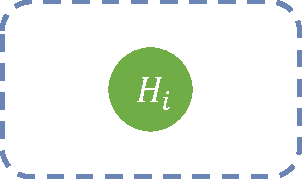
\includegraphics[width=\textwidth,page=1]{abduct1.pdf}
        \caption{仅假设}
    \end{subfigure}\hfill%
    \begin{subfigure}{\firstwidth}
        \includegraphics[width=\textwidth,page=2]{abduct1.pdf}
        \caption{假设和第一个观测}
    \end{subfigure}\hfill%
    \begin{subfigure}{\firstwidth}
        \includegraphics[width=\textwidth,page=3]{abduct1.pdf}
        \caption{假设和第二个观测}
    \end{subfigure}\\[2em]
    \begin{subfigure}{\secondwidth}
        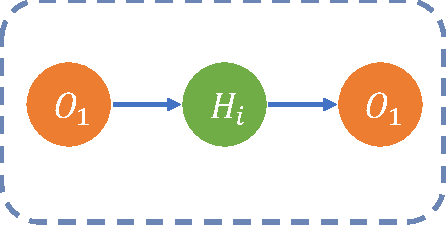
\includegraphics[width=\textwidth,page=1]{abduct2.pdf}
        \caption{线性链}
    \end{subfigure}\hfill
    \begin{subfigure}{\secondwidth}
        \includegraphics[width=\textwidth,page=2]{abduct2.pdf}
        \caption{全连接}
    \end{subfigure}
    \caption{溯因推理的概率模型}
    \label{fig:prob_model}
\end{figure}
这些概率模型给出了在不同条件下来预测$H^*$的表达式。在这些概率模型中,只有全连接模型充分地考虑了各种已知信息的联系,其他的模型或是没有利用完整的观测信息($H$,$H+O_1$,$H+O_2$),或是仅仅分别考虑假设与两个观测的依赖关系(LC)。对于一个好的溯因推理任务,全连接的概率模型(FC)的推理表现应该比其他几种都要高,否则则说明这个推理任务的正确答案对两个观测$O_1$和$O_2$的依赖性不强。所以在之后的实验中,可以用这些概率模型来检验本文提出的视频溯因常识推理任务以及及数据集VideoABC。

\section{常识推理}\label{sec:commonsense}
常识推理(Commonsense Reasoning)顾名思义,是一类在推理过程中需要一些基本常识的推理任务。例如在Zellers~\etal 提出的视觉常识推理\cite{zellers2019recognition}任务中,模型需要通过选择题的形式来回答一些和常识有关的问题,并给出一个做出这个选择的原因。这个任务中的图片来自于影视片段,所以包含大量的人类日常生活中的场景。衡量一个任务是否具有常识性的最简单的方法就是让人类亲自尝试这个任务,并体会在推理的过程中是否用到了常识。从这个的角度来看,教程类视频比较适合来构建和常识推理相关的任务。教程类视频中具有明确的主题和步骤,所以人类能够很容易就可以理解视频的内容,并在多数情况下可以结合生活中的常识判断出不同步骤之间的时序关系。例如在买地铁票的视频中,人类甚至不用看到视频的题目,只需要看到售票机就可知道这个视频是在介绍如何买地铁票,并可以根据常识来回忆出买地铁票的步骤。

\section{视频溯因常识推理}\label{sec:definition}

在本节中,我们明确给出视频溯因常识推理任务的定义。视频溯因常识推理构建在溯因推理的架构上(详见第~\ref{sec:abductive}~节)。具体来说,该任务中的观测和假设的构成如下:
\begin{enumerate}
    \item $O_1$和$O_2$分别为一个完整推理过程的开始状态和结束状态的图片;
    \item $\gH=\{H_i\}$为候选的假设集合,其中每个$H_i$由多个视频构成,每个视频代表一个步骤。即
    \begin{equation}
        H_i = \{v_{i1}, v_{i2}, \ldots, v_{il_i}\},
    \end{equation}
    其中$v_{ij}$表示第$i$个假设中第$j$个步骤,$l_i$表示第$i$个假设中的步骤个数。
\end{enumerate}
模型需要根据两个观测信息来从假设集合$\gH$中选出正确的选项。该任务具有以下几个特点:
\begin{enumerate}
    \item 模型的输入只包含视觉信息。与之前视觉问答相关的任务不同,本文提出的\VACR 中没有任何自然语言的输入。也就是说,模型不会从自然语言中直接或间接获取到推理的过程,从而必须自己学会推理的过程。
    \item 复杂的视觉信息。任务中包含的视觉信息都来自于真实世界的图片或视频,包括人类日常生活中的各种复杂的任务,从而需要模型学会理解一些常识。
    \item 明显的时序关系。每一个假设$H_i$中的步骤都具有明显的时序关系。为了取得较好的推理效果,模型需要能够对步骤内和步骤间的时序关系建模。
\end{enumerate}


\begin{figure}
    \includegraphics[width=\textwidth]{demo.pdf}
    \caption{视频溯因常识推理}
    \label{fig:vacr}
\end{figure}
图~\ref{fig:vacr}~展示了\VACR 的一些例子,包含了四种不同的任务可以看到,每个任务中用的已知条件只有开始和结束的两张图片,而中间的步骤是未知的。模型就是要从这两张已知的图片中选出最合适的步骤序列。同时也可以看到,这里的步骤数目是不确定的。因此,模型必须能够具有处理变长度步骤序列的能力才可以在该任务上取得比较好的表现。

由于\VACR 任务是一个建立在真实视觉信息上的推理任务,未来可能具有许多潜在的应用。例如,该任务可能会应用在机器人的决策问题中,尤其是哪些需要与真实世界具有频繁交互的决策任务。机器人首先可以拍照获取初始状态,用户可以给机器人输入一个目标状态,机器人通过搜索的方法可以得到很多种执行步骤。如果机器人可以顺利地完成\VACR 任务,那么它就可以从这些候选步骤序列中选出正确的一个,从而完成决策。

% !TeX root = ../main.tex

\chapter{VideoABC 数据集}\label{cha:VideoABC}
VideoABC(Video ABductive Commonsense Reasoning)是专门为视频溯因推理任务而设计的一个数据集。该数据集以教程类视频数据集COIN\cite{tang2019coin}为基础进行二次标注进而构建而成。基于COIN数据集来构建VideoABC的原因主要有以下几点:
\begin{enumerate}
    \item COIN数据集是一个教程类视频的数据集,具有明确的步骤划分,每个步骤都是一个将对完整而独立的动作,适合于\VACR 的任务设定;
    \item COIN数据集中的步骤具有很强的时序关系,适合用来构建时序上的视觉推理任务;
    \item COIN数据集中的视频都来自于真实世界,从而需要模型具有对常识的理解能力;
    \item COIN 数据集是目前公开数据集中视频数目最多(11,827个),视频总时长最长(超过476h),视频种类最多(180类)。所以,以COIN为基础构建数据集,可以使得训练出来的模型适应于多种日常生活场景中的推理任务。
\end{enumerate}

本章将详细介绍 VideoABC数据集的构建方式,包括数据的二次标注,数据集的构建,以及难分样本的挖掘。最后将给出VideoABC数据集的一些例子以及统计数据。
\section{数据标注}
\subsection{标注规则}
VideoABC 数据集基于COIN数据集构建,原始的COIN数据集中已经包含了每个步骤的名称以及时间区间的标注,然而COIN的每个视频中可能会出现动作或场景的不连续。二次标注的目的就是通过标注切分点,保证切分后的每个视频的连续性。例如在一个换轮胎的视频中可能包括了多次完整的换轮胎操作,而这每一次的换轮胎操作是互相独立的,属于不同的推理过程,所以应该在相邻的两次换轮胎的操作中间标注一个切分点。再比如在冰壶比赛的视频中,包含了很多轮比赛,而这些比赛是由不同的国家代表队完成的,此时则应该在不同轮比赛之间标注切分。

为了简化表达,本节中对于步骤序列采用以下的记号:
\begin{enumerate}
    \item 用不同的字母表示不同类型的步骤。例如$A$和$B$就表示两种不同的步骤;
    \item 用多个字母相乘来表示一个步骤序列。例如$ABC$表示依次执行$A$步骤、$B$步骤和$C$步骤;
    \item 重复的动作用连乘符号$\prod$来表示。例如$\prod_{i=1}^{2}(BC)$表示步骤序列$BCBC$;
    \item 如果重复的步骤前后具有关联,则对这些步骤增加下角标。例如$\prod_{i=1}^{2}(B_iC_i)$表示步骤序列$B_1C_1B_2C_2$。这里虽然$B_1$和$B_2$属于同样的步骤,但是$B_2$的完成依赖于$B_1$的完成。
\end{enumerate}


\begin{table}[htbp]
    \caption{特殊情况的标注规则}
    \label{tab:anno_rule}
    \begin{tabu}to\textwidth{XXX[2]}\toprule
        步骤形式 & 是否切分 & 原因\\\midrule
        $A\prod_{i=1}^{n}(BC)D$ & \xmark & 整体应该看做一次任务\\
        $\prod_{i=1}^{n}(B_iC_i)$ & \xmark & 重复的动作之间具有连续性\\
        $\prod_{i=1}^{n}(BC)$ & \cmark & 重复的动作之间相互独立\\\bottomrule
    \end{tabu}
\end{table}

在实际标注中,我们发现会有一些复杂的情况,即使存在一些重复的步骤,也不应该标注切分点。经过分析之后为这些情况制定了标注规则如表~\ref{tab:anno_rule}~所示。需要注意的是,这里的重复单元为两个步骤$BC$只是为了表述方便,实际情况中可能为任意步骤的重复单元。下面对这些特殊情况进行详细的解释。
\begin{enumerate}
    \item $A\prod_{i=1}^{n}(BC)D$ 中,虽然$BC$重复了很多次,但是由于具有开始步骤$A$和结束步骤$D$,意味着从$A$到$D$才是一个完整的任务,所以不添加任何切分点;
    \item $\prod_{i=1}^{n}(B_iC_i)$ 中,重复的动作前后具有连续性。例如在贴墙纸的视频中,一面墙需要贴许多张墙纸,每一次贴墙纸是一个重复步骤,但是后一次与前一次之前存在连续性,总体上的任务应该是包含了每一次的贴墙纸。所以,这种情况下不需要标注切分点;
    \item $\prod_{i=1}^{n}(BC)$ 中,重复的动作前后不具有连续性。例如在制作工艺品的视频中,如果制作者一共制作了多个工艺品,则每个制作过程是独立的,所以应该将它们切分开来。
\end{enumerate}

以上在实际的标注过程中,还可能遇到一些其他类型的步骤形式,不过总体上把握一个原则,即保证将所有的不连续点切分开来,即可解决大部分的情况。

\subsection{标注网站}
为了加速标注,本文开发了一个标注网站,允许多名标注员同时操作。本节中将详细介绍标注网站的设计。

标注界面如图~\ref{fig:anno_tool}~所示,可以看到整个界面主要由六个部分构成:

\begin{figure}[htbp]
    \centering
    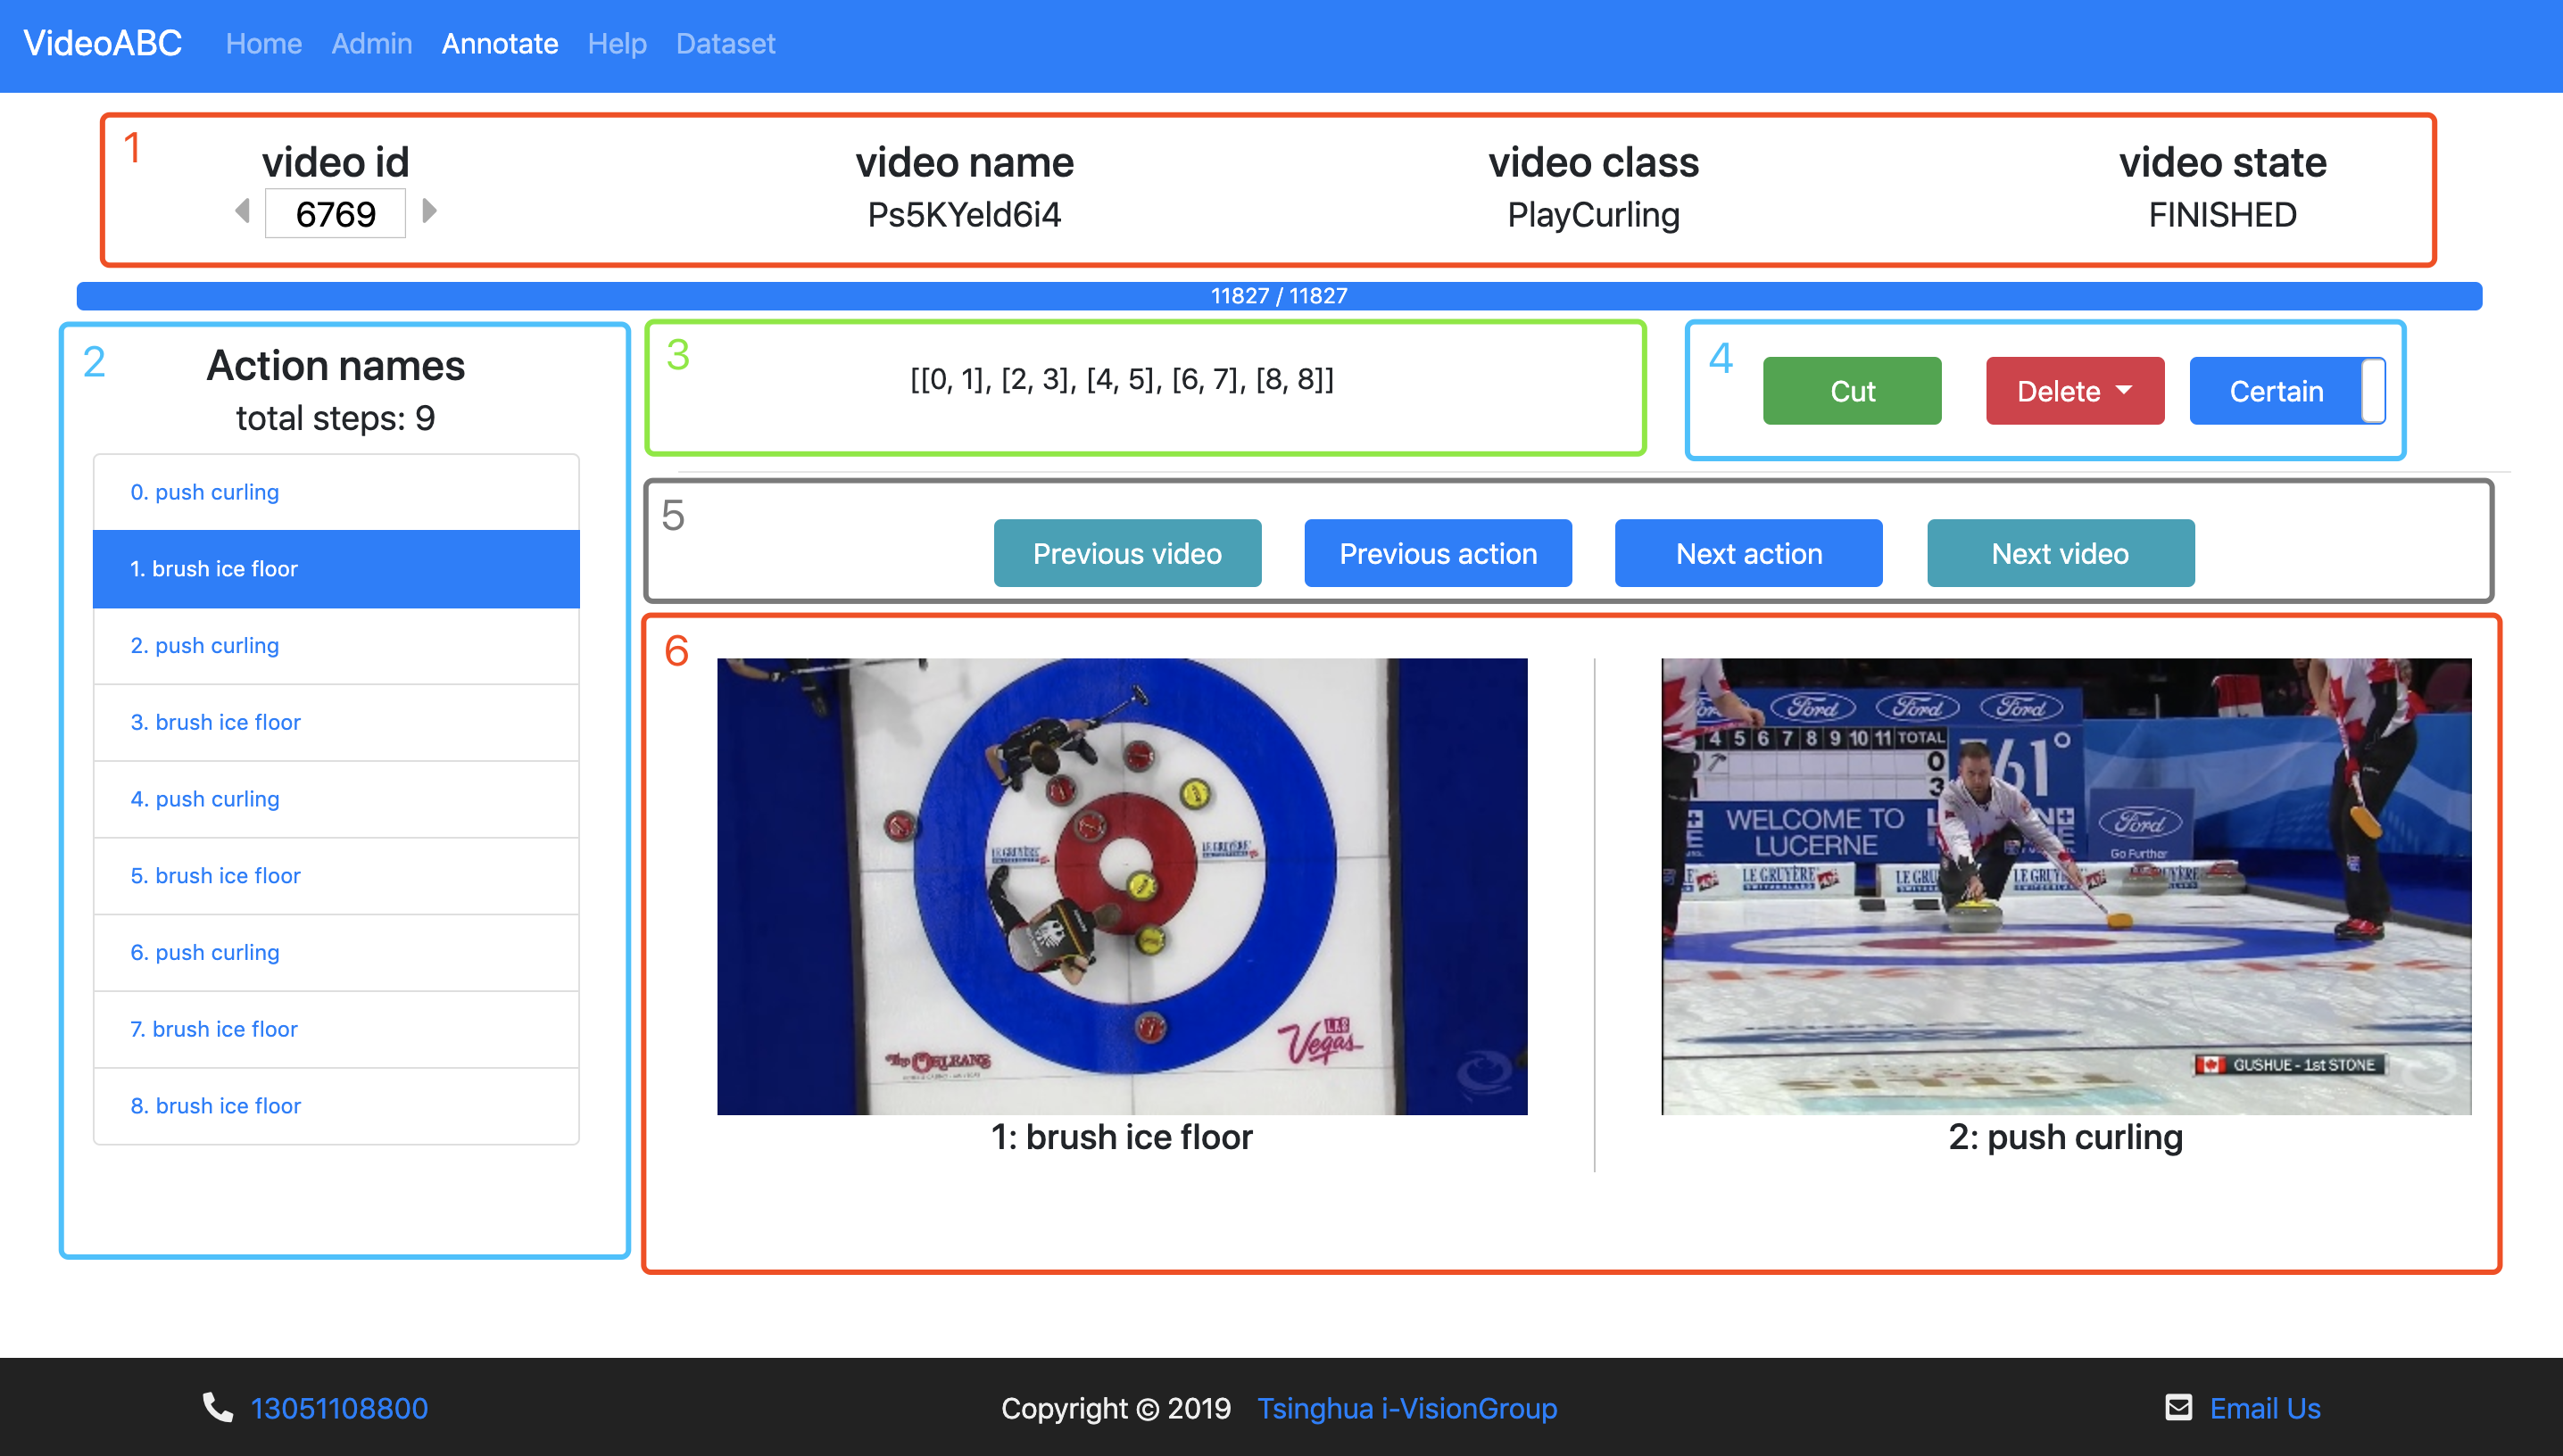
\includegraphics[width=\textwidth]{anno_tool.png}
    \caption{标注界面}
    \label{fig:anno_tool}
\end{figure}

\begin{enumerate}
    \item 基本信息区。显示了视频序号,视频名称、视频种类和视频状态。其中视频的序号是该视频在总视频中的序号,范围是1到11827(视频总数),视频名称为该视频在COIN数据集中原始的名称(来自于Youtube中的视频id),视频种类指的是该视频中的任务类型,视频状态分为三种:未标注,标注中,已标注。
    \item 动作列表区。显示了该视频中所有步骤的动作名称,以及动作总数。当前的步骤用蓝色背景标出,标注员可以点击某个步骤快速到达该步骤。
    \item 切分结果区。以列表的形式显示了当前的切分结果,该列表中的每个元素为一个闭区间,表示了每个切分后的视频区间。例如[[0, 1], [2, 3]]表示在步骤1和步骤2中间存在一个切分点。需要注意的是,这里所有的步骤序号都是从0开始计算的。
    \item 编辑区。包括三个控件:切分按钮、删除按钮、确定性开关。
    \begin{enumerate}
        \item 切分按钮:点击后会在当前步骤和下一步骤中间添加一个切分点。
        \item 删除按钮:点击后会出现一个下拉菜单,标注员可以指定删除某一个切分点或者删除所有的切分点。
        \item 确定性开关:用来表示对当前视频标注结果是否确定,默认为开启状态(确定)。一旦标注员将其切换到关闭状态(不确定)时,界面下方会出现一个文本框,可以在其中填写不确定的理由。这样我们可以在最后统一处理有疑问的视频。
    \end{enumerate}
    \item 导航区。包括四个按钮,分别为上一视频、下一视频、上一步骤、下一步骤。
    \item 关键帧区。展示了当前动作和下一动作的关键帧。由于标注的目标是找到视频中的不连续点,这里显示的是当前步骤的最后一帧和下一步骤的第一帧。如果当前步骤后存在切分点,这两张图片之间会显示一条浅灰色的竖线(如图~\ref{fig:anno_tool}~所示)。
    
\end{enumerate}


\begin{table}[!h]
    \caption{标注网站的键盘快捷键}
    \begin{tabu}to\textwidth{X[c]X[c]}\toprule
        键盘按键 & 功能\\\midrule
        \keys{A}	& 下一步骤\\
        \keys{S}	& 上一步骤\\
        \keys{F}	& 第一个步骤\\
        \keys{E}	& 最后一个步骤\\
        \keys{0}~$\sim$~\keys{9}	& 跳转到第$i$个步骤($i\in[0, 9]$)\\
        \keys{V}	& 下一视频\\
        \keys{B}	& 上一视频\\
        \keys{\arrowkeyleft}    & 上一视频 (以视频序号计算)\\
        \keys{\arrowkeyright} & 下一视频 (以视频序号计算)\\
        \keys{C}	& 切分\\
        \keys{R}	& 跳转到下一个状态为“标注中”的视频\\\bottomrule
    \end{tabu}
\end{table}

在实际标注的过程中,标注员可以先通过视频类型和左侧的动作列表中来了解该视频中任务的特点。对于每个视频,标注员在多个情况下都可以直接通过动作列表中的文本来找到重复的步骤单元,从而能够快速定位切分点并标注。另外,为了加速标注,一些常用的操作都绑定了键盘快捷键,包括步骤和视频的跳转、切分点的编辑等等。需要注意的是,这里的快捷键“V”表示的“下一视频”指的是下一个未标注的视频。如果想跳转到按照视频序号的下一视频应该按向右方向键。

为了统一标注的标准,标注网站的导航栏中设置了“Help”标签页,用来显示帮助信息,其中包括了标注规则、标注方法和标注快捷键,如图~\ref{fig:help}~所示。

\begin{figure}[htbp]
    \centering
    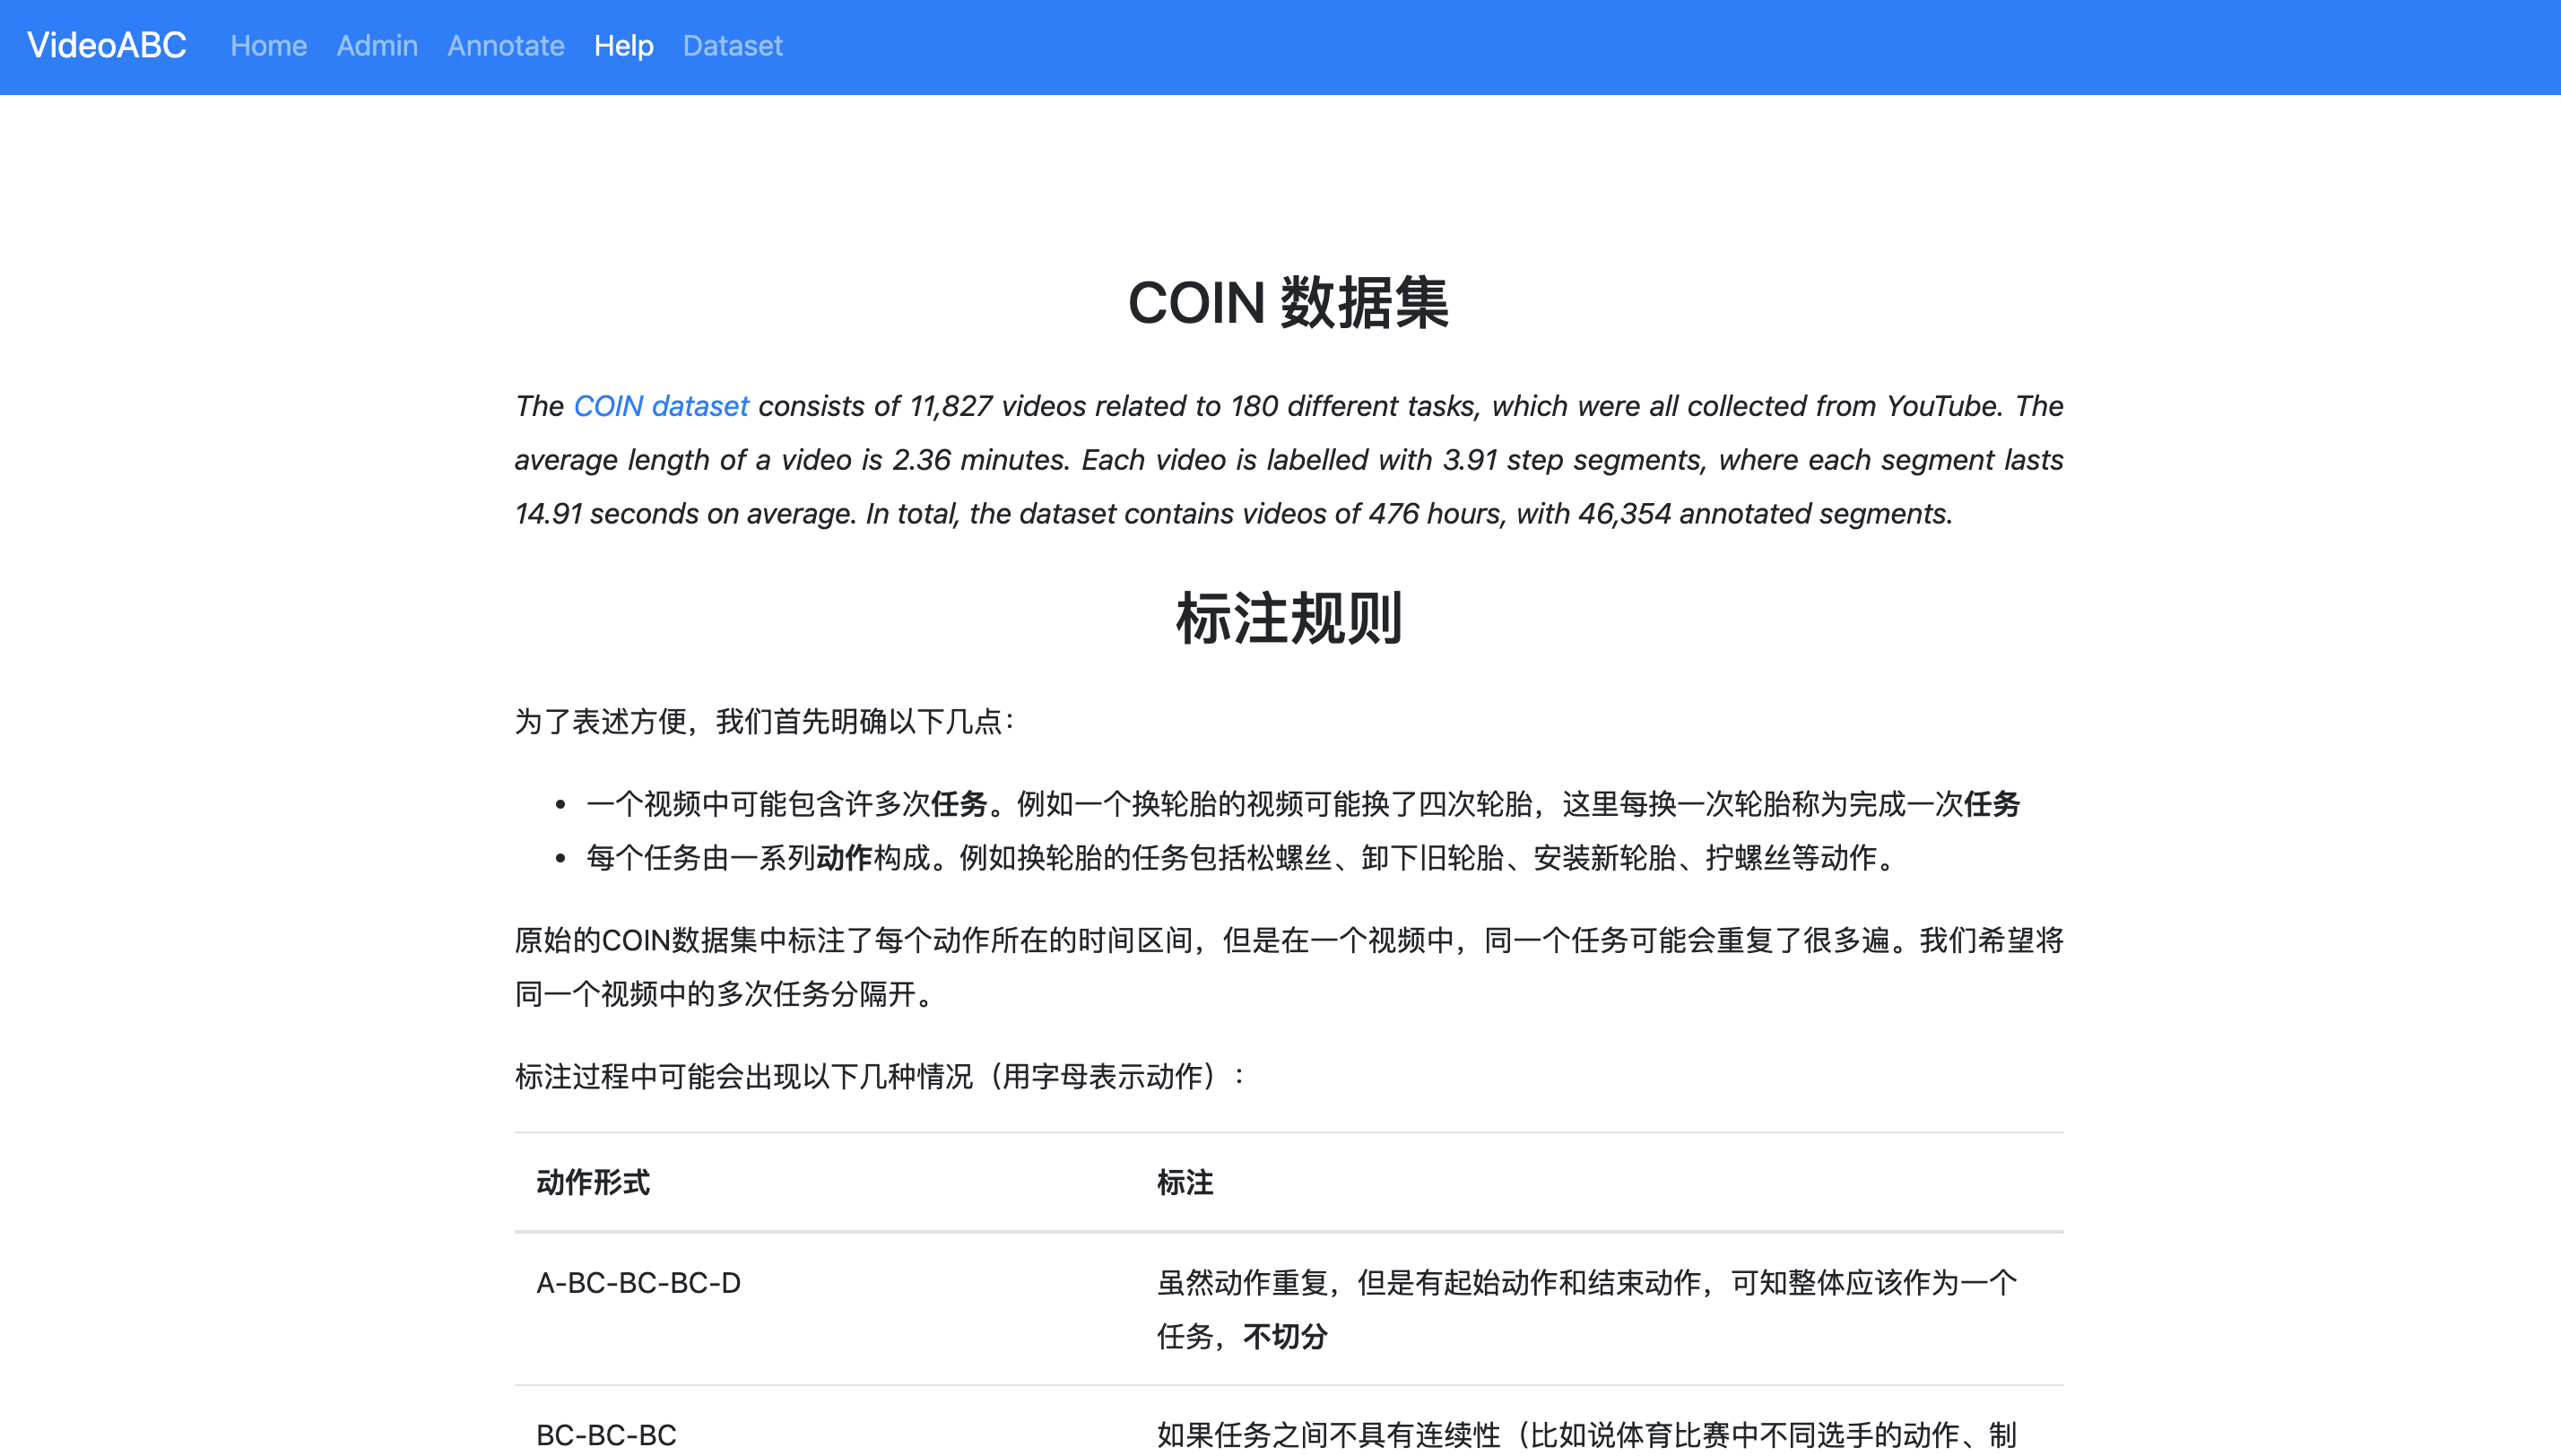
\includegraphics[width=\textwidth]{help.png}
    \caption{标注网站的帮助页面}
    \label{fig:help}
\end{figure}

\subsection{标注网站的实现细节}
本节将详细介绍标注网站的实现细节。
\subsubsection{后端}
标注网站的后端基于Django\cite{django}框架构建。一个Django工程中可以包含多个应用(app),例如本节中介绍的标注工具就是一个应用,我们将其命名为anno(annotation)。anno 文件夹下的目录如下(仅列出主要的文件和目录):
\begin{enumerate}
    \item anno/
    \begin{enumerate}
        \item models.py
        \item views.py
        \item urls.py
        \item static/
        \item templates/
        \item ...
    \end{enumerate}
\end{enumerate}
其中,models.py 中定义了数据结构,urls.py 中定义了各个网页的url,views.py 中定义了每个网页的传入内容和跳转关系,templates 目录中的 HTML 模板用来渲染每个网页,static 目录中用来存放一些固定不变的文件(如图片、视频、CSS 等等)。下面介绍后端的一些重要组成部分,包括数据结构、URL定义和页面跳转逻辑,以及它们的实现方式。

\paragraph{数据结构} 首先需要定义数据结构,即标注结果的存储方式。由于我们的标注是以视频为单位进行的,这里的数据结构也应该以视频为单位。具体来说,我们定义Video类如表~\ref{tab:video_vars}~所示。大部分的内容在表中已经表达得很清楚,但仍有一些需要明确:
\begin{enumerate}
    \item action\_ids 是指该视频中的动作在COIN数据集中\emph{所有}动作的序号,不同的动作用逗号分隔开。
    \item cut\_points 中不同的切分点用逗号分隔,例如“1,2,5”表示在步骤1、步骤2、步骤5后添加切分点。
    \item note 只在 certainty 被置为False时才可写入。
    \item prev\_vid 是指当前编辑视频之前所编辑的视频的序号。
\end{enumerate}

Video类定义在models.py中,Django框架可以自动为其链接到数据库(本文使用SQLite数据库),所有的Video对象被保存在数据库中的一张表中,数据域与成员变量相对应。
\begin{table}
    \caption{Video类成员变量}
    \label{tab:video_vars}
    \begin{tabu}to\textwidth{XXX}\toprule
        变量名称 & 变量类型 & 变量含义\\\midrule
        video\_name & 字符串 & 视频名称\\
        video\_class  & 字符串 & 视频类型\\
        steps & 小正整型 & 步骤总数\\
        action\_ids & 字符串 & 动作序号\\\midrule
        cut\_points & 字符串 & 切分点\\
        state & 小正整型 & 视频状态\\
        certainty & 布尔型 & 确定性\\
        note & 字符串 & 备注\\
        prev\_vid & 小正整型 & 上次编辑的视频序号\\
        checkpoint & 小正整型 & 上次编辑的步骤序号\\\bottomrule
    \end{tabu}
\end{table}

\paragraph{URL 定义} 表~\ref{tab:urls}~中给出了 anno 中用到的主要URL定义、绑定的函数以及对应的含义。Django使用URL模式(URL patterns)的方法来定义一个通用的格式(相对路径),并对这个URL模式绑定一个函数(在views.py中定义),具体访问URL的时候再将URL中的参数传入到函数里可进行处理。例如,如果app部署的根路径为“localhost:8888/anno”,则访问链接“localhost:8888/anno/1/0” 时内部的实现逻辑如下:
\begin{enumerate}
    \item Django按照格式和变量类型从anno中所有预定义的URL模式中匹配“1/0”,发现只有 “<int:video\_id>/<int:start\_step>”符合。
    \item 通过该URL模式,找到了绑定的函数views.anno函数。
    \item 将“video\_id=1, start\_step=0”作为参数传入views.anno函数调用。
    \item views.anno 函数中通过访问数据库得到需要显示的内容,并传给HTML模板渲染。
\end{enumerate}

可以看到,表~\ref{tab:urls}~中除了标注界面,其他的URL模式都属于用来过渡的URL。这些URL模式的设置是为了方便通过调用函数的形式与数据库交互,最终都会回到标注界面。

\begin{table}
    \caption{URL模式的定义}
    \label{tab:urls}
    \begin{tabu}to\textwidth{X[1.5]XX}\toprule
        URL 模式 & 绑定函数 &含义\\\midrule
        <int:video\_id>/<int:start\_step> & views.anno & 标注界面\\ 
        start/ & views.start &开始(过渡)\\
        resume/& views.resume &恢复(过渡)\\
        <int:video\_id>/navigate & views.navigate &导航(过渡)\\
        <int:video\_id>/edit & views.edit &编辑(过渡)\\\bottomrule
    \end{tabu}
\end{table}
\paragraph{页面跳转逻辑} 表~\ref{tab:urls}~中已经给出了URL模式的定义,下面介绍它们之间的页面跳转逻辑。
\begin{enumerate}
    \item 访问标注界面时,后端会调用 views.anno 函数,根据video\_id 从数据库中读取对应视频条目,根据start\_step 选定当前步骤,将所有需要显示的信息(视频基本信息、关键帧路径、标注进度等)传入HTML模板中渲染。
    \item 点击动作列表区的步骤,会改变当前的步骤序号并重新加载标注页面。
    \item 按下导航区的某个按钮时会发送表单到 <int:video\_id>/navigate ,进而调用views.navigate 函数。在函数内部通过读取表单信息,确定导航后的视频序号、步骤序号,再重定向到标注页面。
    \item 按下编辑区的按钮时会发送表单到<int:video\_id>/edit,并调用views.edit 函数。函数内部会读取表单信息,决定执行添加切分点、删除切分点或者改变确定性的操作。编辑结束后再重定向回标注页面。
   \item 执行步骤之间的导航操作时,views.navigate 函数会将当前的步骤记录在checkpoint中,便于记录进度。
   \item 点击下一视频按钮时,将当前视频状态更改为标注完成,并选择一个未标注的视频作为下一视频,将下一视频的“prev\_id”变量更改为当前视频的序号。
   \item 按下快捷键“R”时,跳转到resume/ 并调用 views.resume 函数,寻找数据库中处于“标注中”状态的视频并跳转到该视频的标注界面。
   \item 在标注网站的主页(图~\ref{fig:anno_index}~)中有两个按钮,分别为继续上一标注(Continue)和开始新标注(Start new)。若选择继续上一标注,则跳转到resume/页面;若选择开始新标注,则跳转到start/页面,通过调用views.start 函数,在数据库中选择一个未标注过的视频并跳转到该视频的标注页面。
\end{enumerate}

以上的这些跳转逻辑在实现标注功能的同时保证了线程安全,确保可以多个标注员同时标注而不发生冲突。其中视频状态的设计相当于加锁,保证一位标注员在对某个视频标注的过程中其他标注员不会访问到同样的视频。

\begin{figure}[htbp]
    \centering
    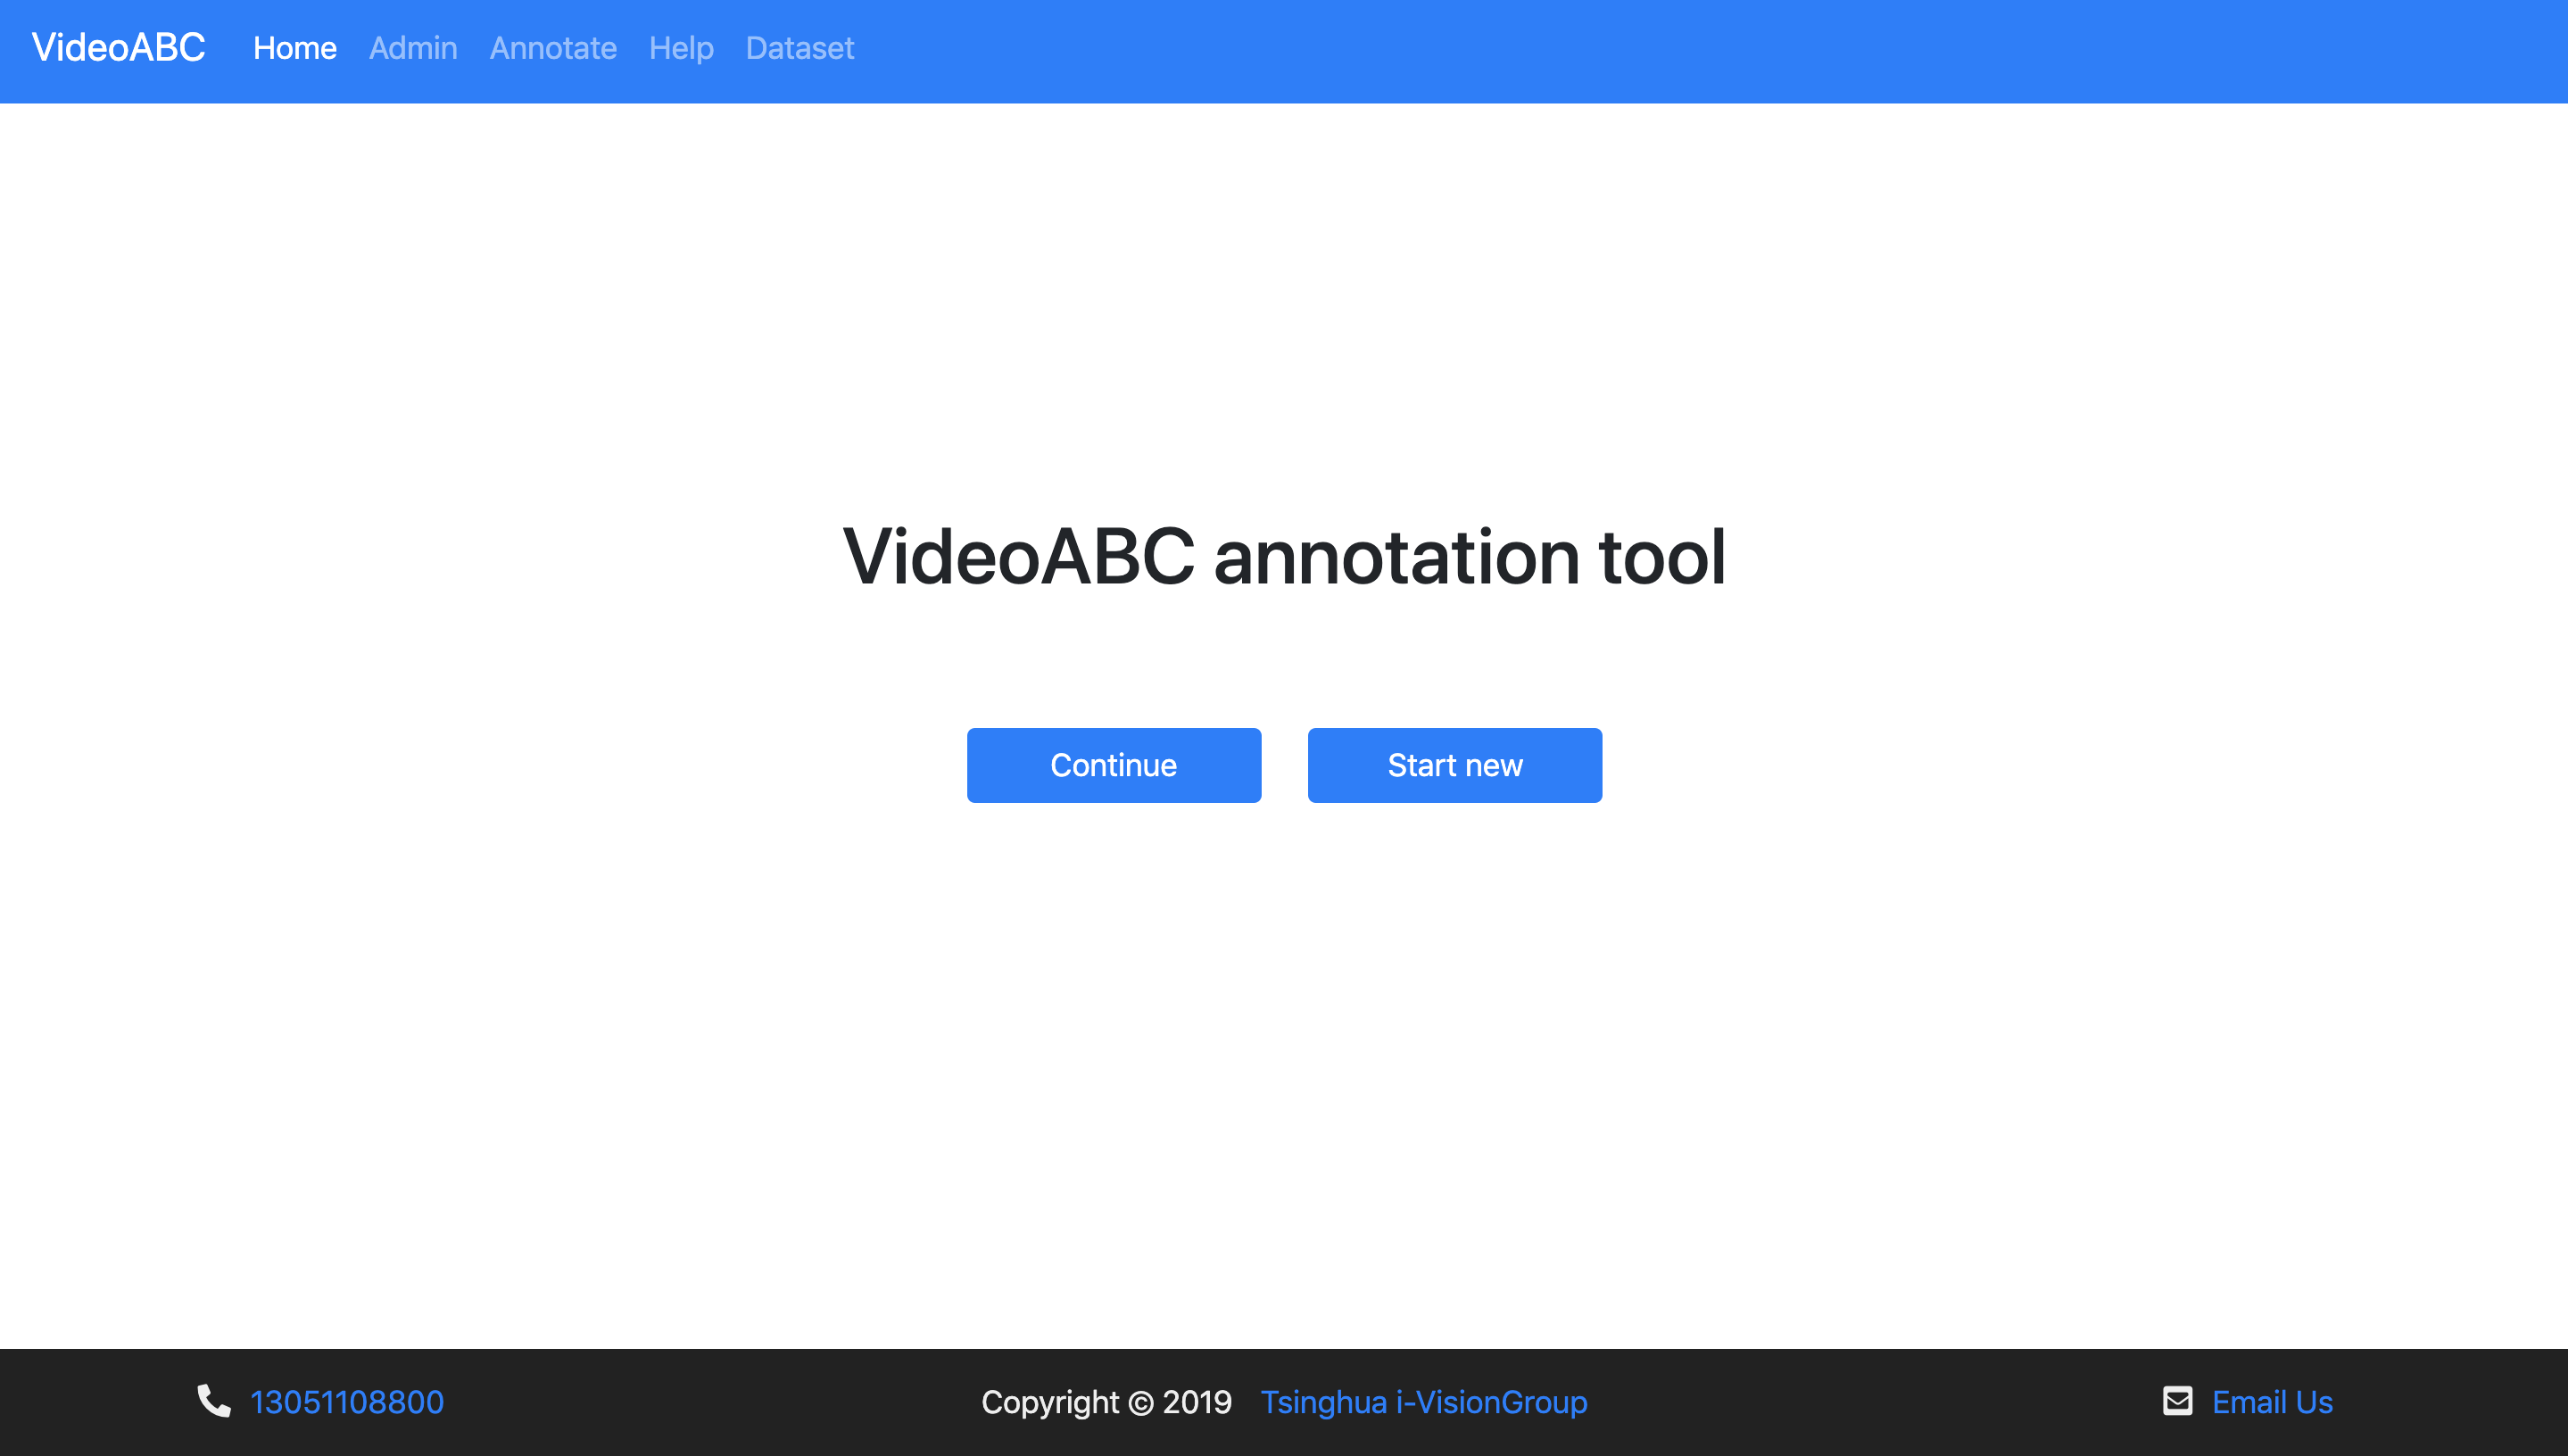
\includegraphics[width=\textwidth]{index.png}
    \caption{标注网站主页}
    \label{fig:anno_index}
\end{figure}
\subsubsection{前端}
标注网站的前端使用HTML+CSS+JavaScript 构建。其中HTML负责基本排版,CSS负责样式渲染,JavaScript用来实现各种快捷键操作。为了统一风格,本文使用了Bootstrap\cite{bootstrap}库完成了大部分的排版和渲染。使用Bootstrap 有以下几个好处:
\begin{enumerate}
    \item 包括了大量的预定义样式,例如按钮、导航栏、表单等等,可节省大量的CSS代码编写量。且风格统一,简洁而不失美观。
    \item 调用十分方便,只需在代码中添加几行就可以使用。
    \item 复用性强,目前很多网站中都在使用Bootstrap框架,所以大部分的浏览器中都已经预先下载过Bootstrap中的资源,避免了资源文件的重复下载。
    \item 具有多种使用的便于使用的布局工具,例如流动性容器可以使控件根据屏幕大小自动调整,便于从不同的客户端访问标注网站。
\end{enumerate}

\section{数据集构建}
\subsection{视频切分与筛选}
\label{sec:filter}
在标注数据的过程中,我们已经在视频中的不连续位置标记了切分点,但是即使这样,切分后的视频中的步骤数目仍然相差很大。为了便于处理,我们需要设置步骤数目的限制。另外,我们还需要保证训练集和测试集中的视频片段分布的均匀性。设原始的视频数据集为$\gD=\{D_i\}$,则视频切分与筛选的算法如下:
\begin{enumerate}
    \item 使用标注的切分点将视频切分,得到数据集$\gD'$;
    \item 给定最小步骤数$m=2$和最大步骤数$M=6$;
    \item 利用$m$和$M$对$\{D_i'\}$进一步处理,即对步骤数大于$M$的进行再次切分,对步骤数少于$m$的直接去除,得到数据集$\gD''$;

\end{enumerate}
经过上述算法后,我们已经得到了清洗后的数据集$\gD''$,其中每个样本中的步骤数目都在$m$到$M$之间。基于$\gD''$的每个样本,可以按照如下步骤来构建正确选项:
\begin{enumerate}
    \item 对每个步骤按照COIN的原始标注的时间区间抽取16帧;
    \item 第一个步骤的第一帧作为$O_1$,最后一个步骤的最后一帧作为$O_2$;
    \item 截取每个步骤的\emph{中间}8帧作为最终使用的视频片段,构成正确假设$H_+$。
\end{enumerate}

上述的做法保证了两个观测$O_1$和$O_2$不会直接出现在$H_+$的帧中。否则如果$H_+$里直接使用16帧,或等间隔抽8帧都会出现这种情况,导致模型只需要做简单的比对就能得出答案。

接下来对数据集进行划分。定义训练集比例$\alpha$,划分训练集和测试集,保证:
\begin{enumerate}
    \item $\gD''$中来自于同一个原始视频的必须同时被划分到训练集或测试集;
    \item 同一类别的视频中,训练样本的比例尽可能接近$\alpha$。
\end{enumerate}
至此,我们已经得到了训练集和测试集的所有观测和正确假设。
\subsection{错误假设生成}
本节介绍如何根据正确假设来生成错误的假设集合$\gH_-$。VideoABC数据集中共包括四种错误类型:
\begin{enumerate}
    \item 删除(remove)一个步骤;
    \item 交换(swap)两个步骤;
    \item 插入(insert)一个步骤;
    \item 替换(replace)一个步骤。
\end{enumerate}
正是因为有这几种错误类型,我们在之前对视频切分和筛选时才指定了一个最小步骤数$m=2$,否则swap和remove两种错误类型将不存在,insert则可以通过判断步骤数简单排除,只剩下replace 的错误类型可供选择。对于每个问题,我们会均匀生成各种错误类型的选项,从中选取三个,与正确选项一起,构成一个四选一的选择题。
\subsection{难分选项挖掘}
构建VideoABC时的一个关键的地方在于能够生成出高质量的干扰选项,从而使得任务更有挑战,更能筛选出推理能力强的模型。为了去除过于明显的错误假设,本文使用了难分选项挖掘(Hard Choice Mining)的方法来提高难度。具体步骤如下:
\begin{enumerate}
    \item 使用上一节的方法生成错误选项得到初始的数据集;
    \item 在初始的数据集上训练一些基础模型,并选出表现最好的;
    \item 对每个样本再次生成错误选项,每种类型错误选项生成不超过15个,利用预训练模型选出其中分数最高的3个,构成新的数据集;
\end{enumerate}
通过不断重复上述步骤,最终得到的数据集中的错误选项都是具有一定的干扰性的,从而提高了VideoABC数据集的难度。

\section{VideoABC数据集}
在本章前面几节中,我们已经详细地介绍了VideoABC数据集的构建方式,下面介绍VideoABC中的一些统计数据。
\begin{figure}[htbp]
    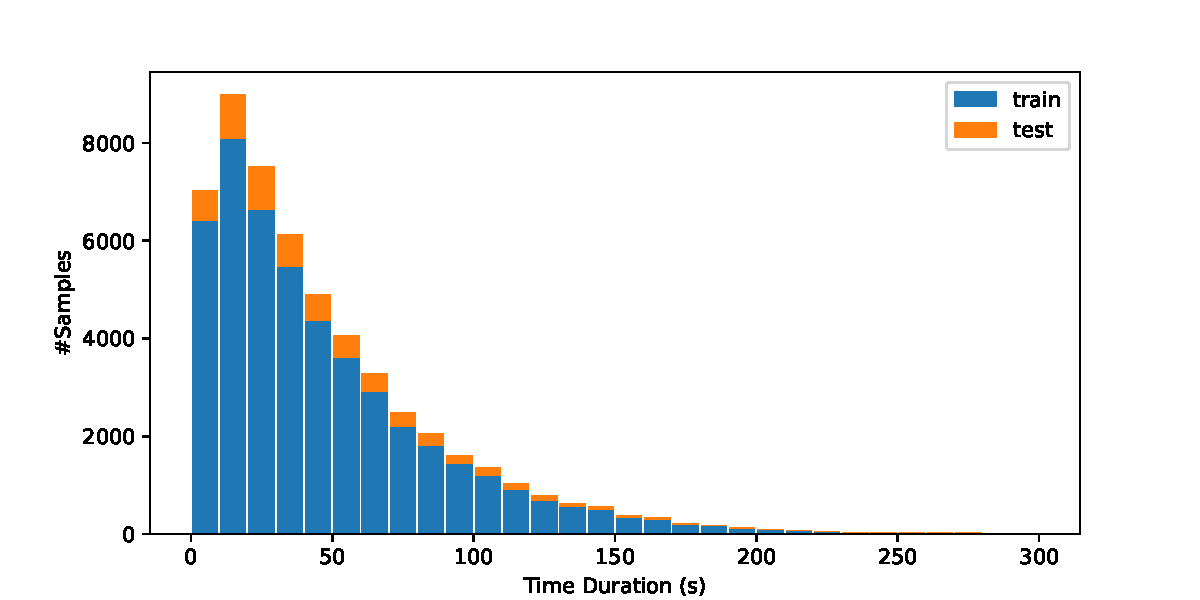
\includegraphics[width=\textwidth]{duration.pdf}
    \caption{VideoABC 的推理时长分布}
    \label{fig:duration}
\end{figure}

图~\ref{fig:duration}~中展示了VideoABC中的推理时长的分布(仅展示0$\sim$300s之间),横坐标为推理时长,纵坐标为选项个数。可以看到VideoABC中的推理时长是一个长尾分布,主要分布在0$\sim$200s之间。可见模型要想在该数据集上取得良好的表现,必须具有能够对长期和短期视觉信息推理的能力。

\begin{figure}[htbp]
    \centering
    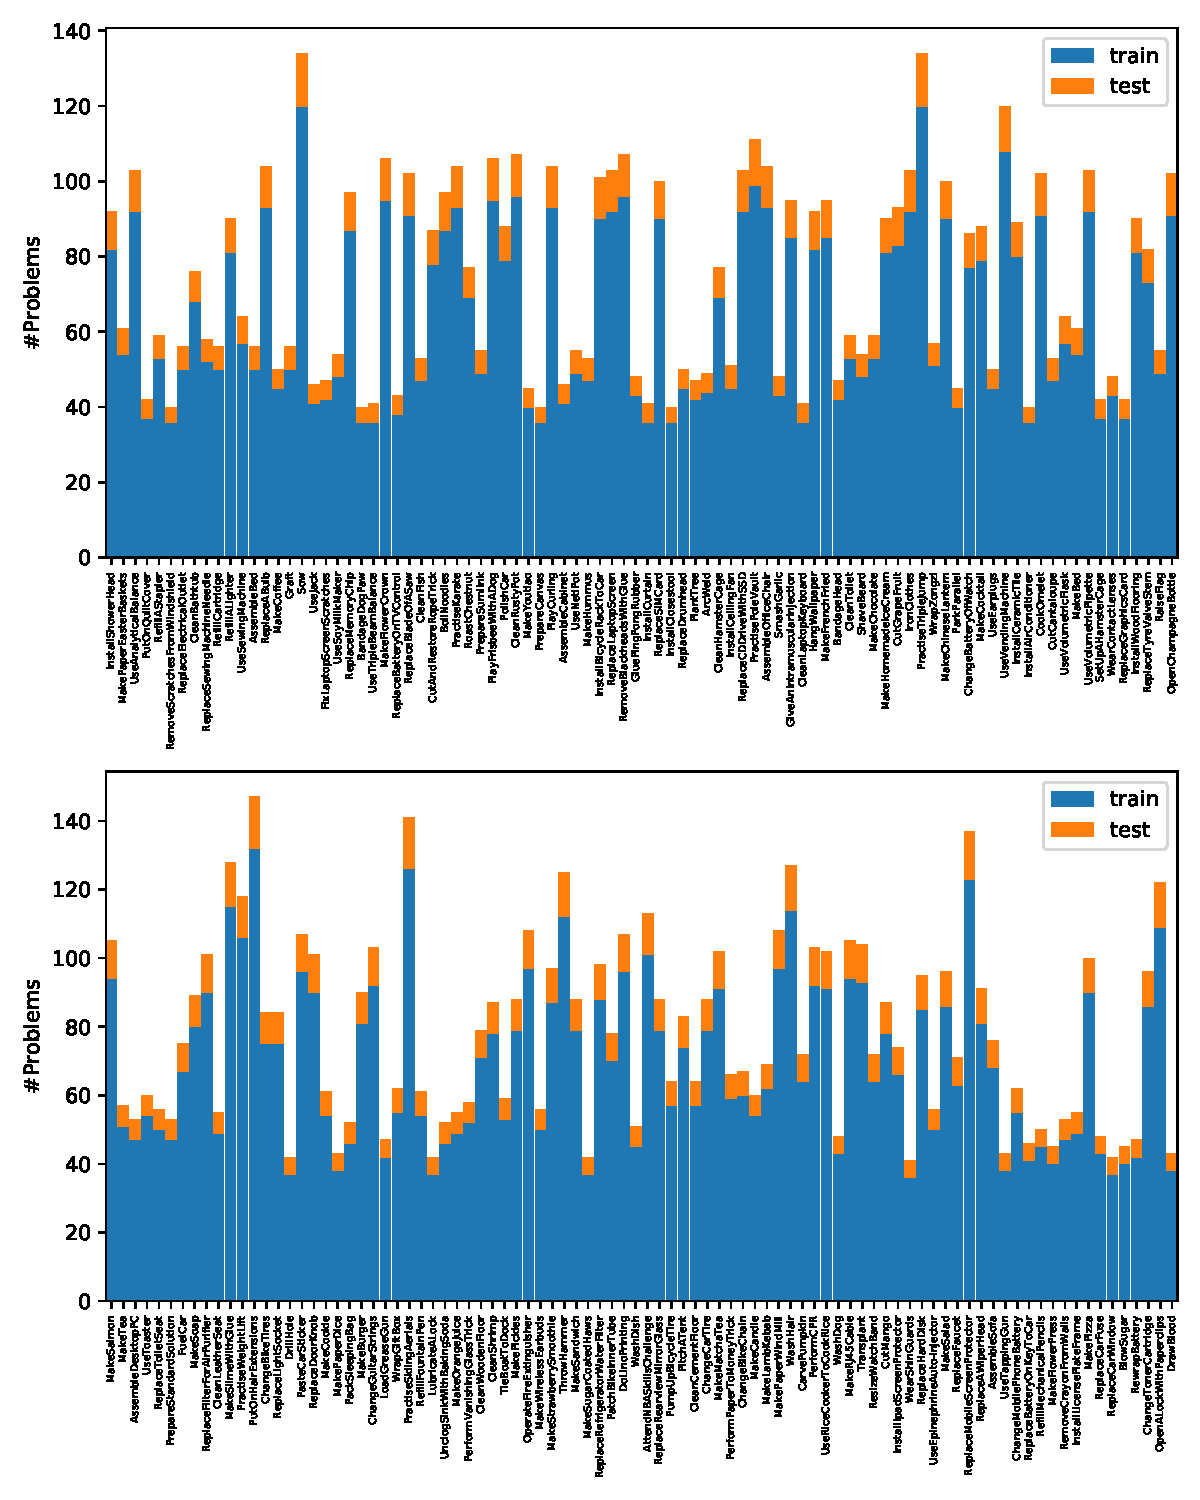
\includegraphics[width=\textwidth]{tasks.pdf}
    \caption{VideoABC 中任务分布}
    \label{fig:tasks}
\end{figure}
图~\ref{fig:tasks}~中展示了VideoABC总的任务种类分布,其中横轴为任务种类,纵轴为对应的问题数。VideoABC中包含180中任务种类(与COIN数据集中的任务种类一致),涵盖生活中的各种场景
从图中可以看出,每种任务种类中训练集的比例均接近90\%。

\begin{figure}[htbp]
    \centering
    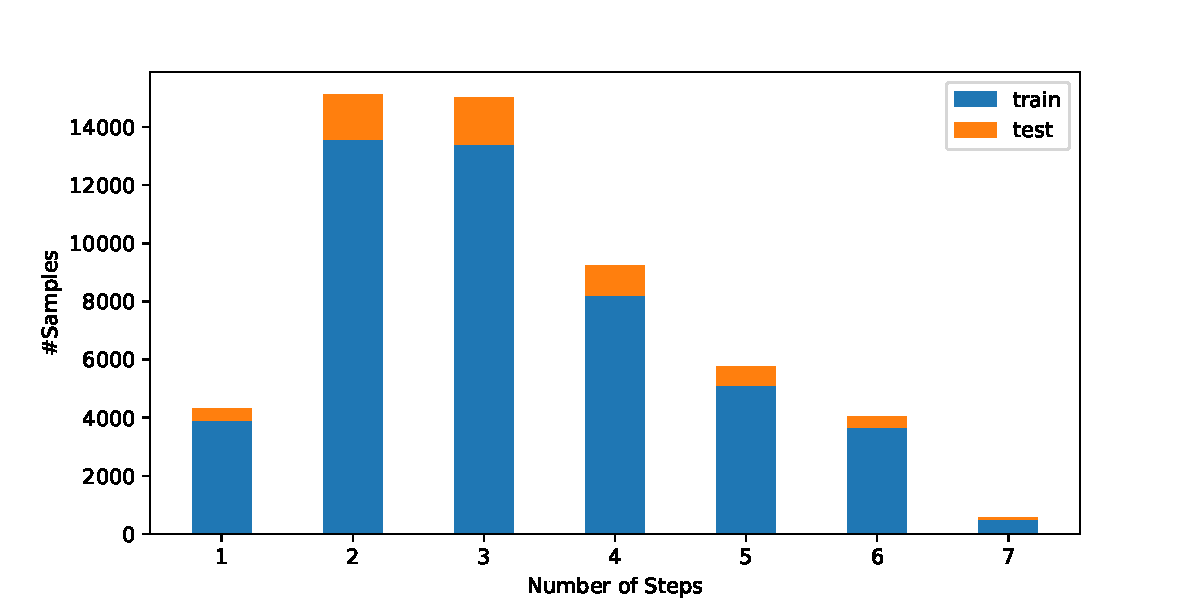
\includegraphics[width=\textwidth{}]{steps.pdf}
    \caption{VideoABC 选项中步骤数分布}
    \label{fig:steps}
\end{figure}

图~\ref{fig:steps}~展示了VideoABC中的步骤数的分布。在第~\ref{sec:filter}~里,我们曾指定了\emph{正确}选项的最小步骤数$m=2$和最大步骤数$M=6$。再将四种错误类型考虑进去,可知\emph{所有}选项的最大步骤数是$M+1=7$(正确选项步骤数为6,错误类型为插入),最小步骤数是$m-1=1$(正确选项步骤数为2,错误类型为删除)。所以可以看到,VideoABC中的步骤数分布在1$\sim$7之间,但是步骤数是1或7的选项都比较少。

\begin{figure}[htbp]
    \centering
    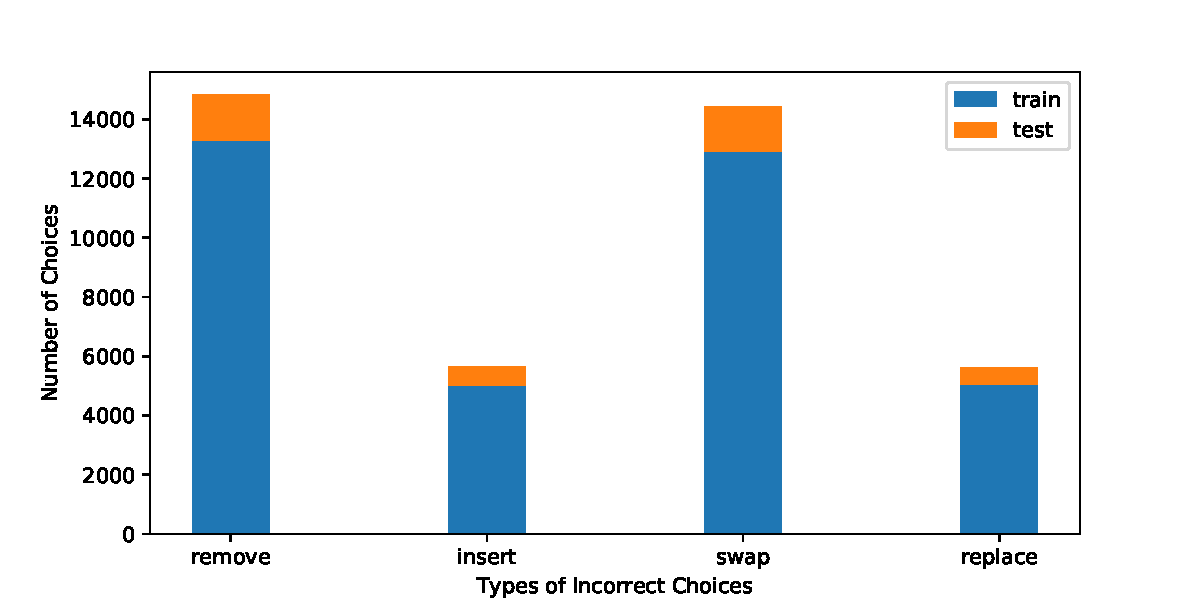
\includegraphics[width=\textwidth]{types.pdf}
    \caption{VideoABC 选项中错误类型的分布}
    \label{fig:wrong_types}
\end{figure}

图~\ref{fig:wrong_types}~中展示了VideoABC选项中错误类型的分布。可以看到,四种类型的错误选项并不是均匀分布,这就体现了难分选项挖掘的作用。经过难分样本挖掘之后,留下来的错误选项都是一些比较具有干扰性的。由此可以看出,删除和交换两种错误类型是比较困难的,而插入和替换两种错误类型是比较简单的。

\begin{table}[htbp]
    \caption{VideoABC的统计数据}
    \label{tab:stat}
    \begin{tabu}to\textwidth{XX}\toprule
        名称 & 统计数据\\\midrule
        原始视频数 & 11,827\\
        任务种类数 & 180\\
        步骤类型数 & 778\\\midrule
        步骤总数 & 46,354\\
        问题总数 & 13,522\\
        训练集问题总数 & 12,086\\
        测试集问题总数 & 1,436\\\midrule
        最大推理时长 & 731s\\
        平均推理时长 & 47s\\\bottomrule
    \end{tabu}
\end{table}

表~\ref{tab:stat}~中展示了VideoABC数据集的一些统计数据。由于VideoABC数据集是基于COIN数据集构建的,VideoABC具有多种多样的任务种类和步骤类型。VideoABC中共有13,522个问题,其中训练集中有12,086个,测试集中有1,436个。另外可以看到,VideoABC中推理时长的范围非常大,最大可达731s,平均推理时长为47s,模型必须能够适应长时间的推理任务才能在VideoABC上取得良好的表现。

\begin{figure}[]
    \begin{subfigure}{\textwidth}
        \centering
        \includegraphics[width=.8\textwidth,page=1]{VideoABC.pdf}
        \caption{}
    \end{subfigure}
    \begin{subfigure}{\textwidth}
        \centering
        \includegraphics[width=.8\textwidth,page=2]{VideoABC.pdf}
        \caption{}
    \end{subfigure}
    \begin{subfigure}{\textwidth}
        \centering
        \includegraphics[width=.8\textwidth,page=3]{VideoABC.pdf}
        \caption{}
    \end{subfigure}
    \begin{subfigure}{\textwidth}
        \centering
        \includegraphics[width=.8\textwidth,page=4]{VideoABC.pdf}
        \caption{}
    \end{subfigure}
    \caption{VideoABC数据集示例}
    \label{fig:illu}
\end{figure}
图~\ref{fig:illu}~展示了VideoABC数据集中的一些例子。在VideoABC数据集中,每个问题中都有一个正确选项和三个错误选项,图~\ref{fig:illu}~中则对每个问题只展示了一个正确选项一个错误选项。其中错误选项的错误类型已经用文字和虚线框标出。在实际的数据集中,每个选项中的步骤其实是一个视频片段,而图中只显示了视频片段的最中间的一帧。图~\ref{fig:illu}~中的四个子图分别对应着四种错误类型:插入、删除、交换、替换。同时,图~\ref{fig:illu}~中的例子属于不同类型的任务(烹饪、小制作、修理、体育运动),由此也可以看出VideoABC数据集中推理场景的多样性。

实验发现,一些最先进的的视频理解模型在VideoABC上都没能取得很好的表现,(具体的实验结果会在第~\ref{cha:experimetns}~章介绍)。为了解决这个问题,我们有必要针对视频溯因推理的特点来重新设计模型结构。
% !TeX root = ../main.tex

\chapter{实验结果}
\section{基准实验}
\section{}
\section{}
% !TeX root = ../main.tex

\chapter{实验结果}\label{cha:experimetns}
本章中列出了VideoABC数据集上的大量的实验结果。首先,本文构建了一个人类水平测试的工具,用来检验人类在VideoABC数据集上的表现(第~\ref{sec:exp:humantest}~节);其次,第~\ref{sec:exp:results}~列出了VideoABC上不同模型的准确率,包括一些目前视频理解方面最先进的模型以及本文提出的HDR Net模型等等。在第~\ref{sec:exp:prob}~中,本文利用第~\ref{sec:abductive}~节中的概率模型来对VideoABC数据集进行检验,证明了观测信息起到了重要作用;最后,第~\ref{sec:exp:ablation}~列出了VideoABC和HDR Net 的一些消融实验的结果。

\section{人类水平测试工具}\label{sec:exp:humantest}
为了检验人类在VideoABC数据集的表现,本文开发了一个人类水平测试工具。与标注工具相同,这个测试工具也是以测试网站的形式实现的,所以可以满足多个测试人员同时答题。本节中将介绍这个测试工具的设计。测试界面如图~\ref{fig:humantest}~所示,整体界面非常简单。测试人员可以看到每个问题中的两个观测和四个假设选项,选中后点击提交按钮即可切换到下一题。
\begin{figure}[htbp]
    \centering
    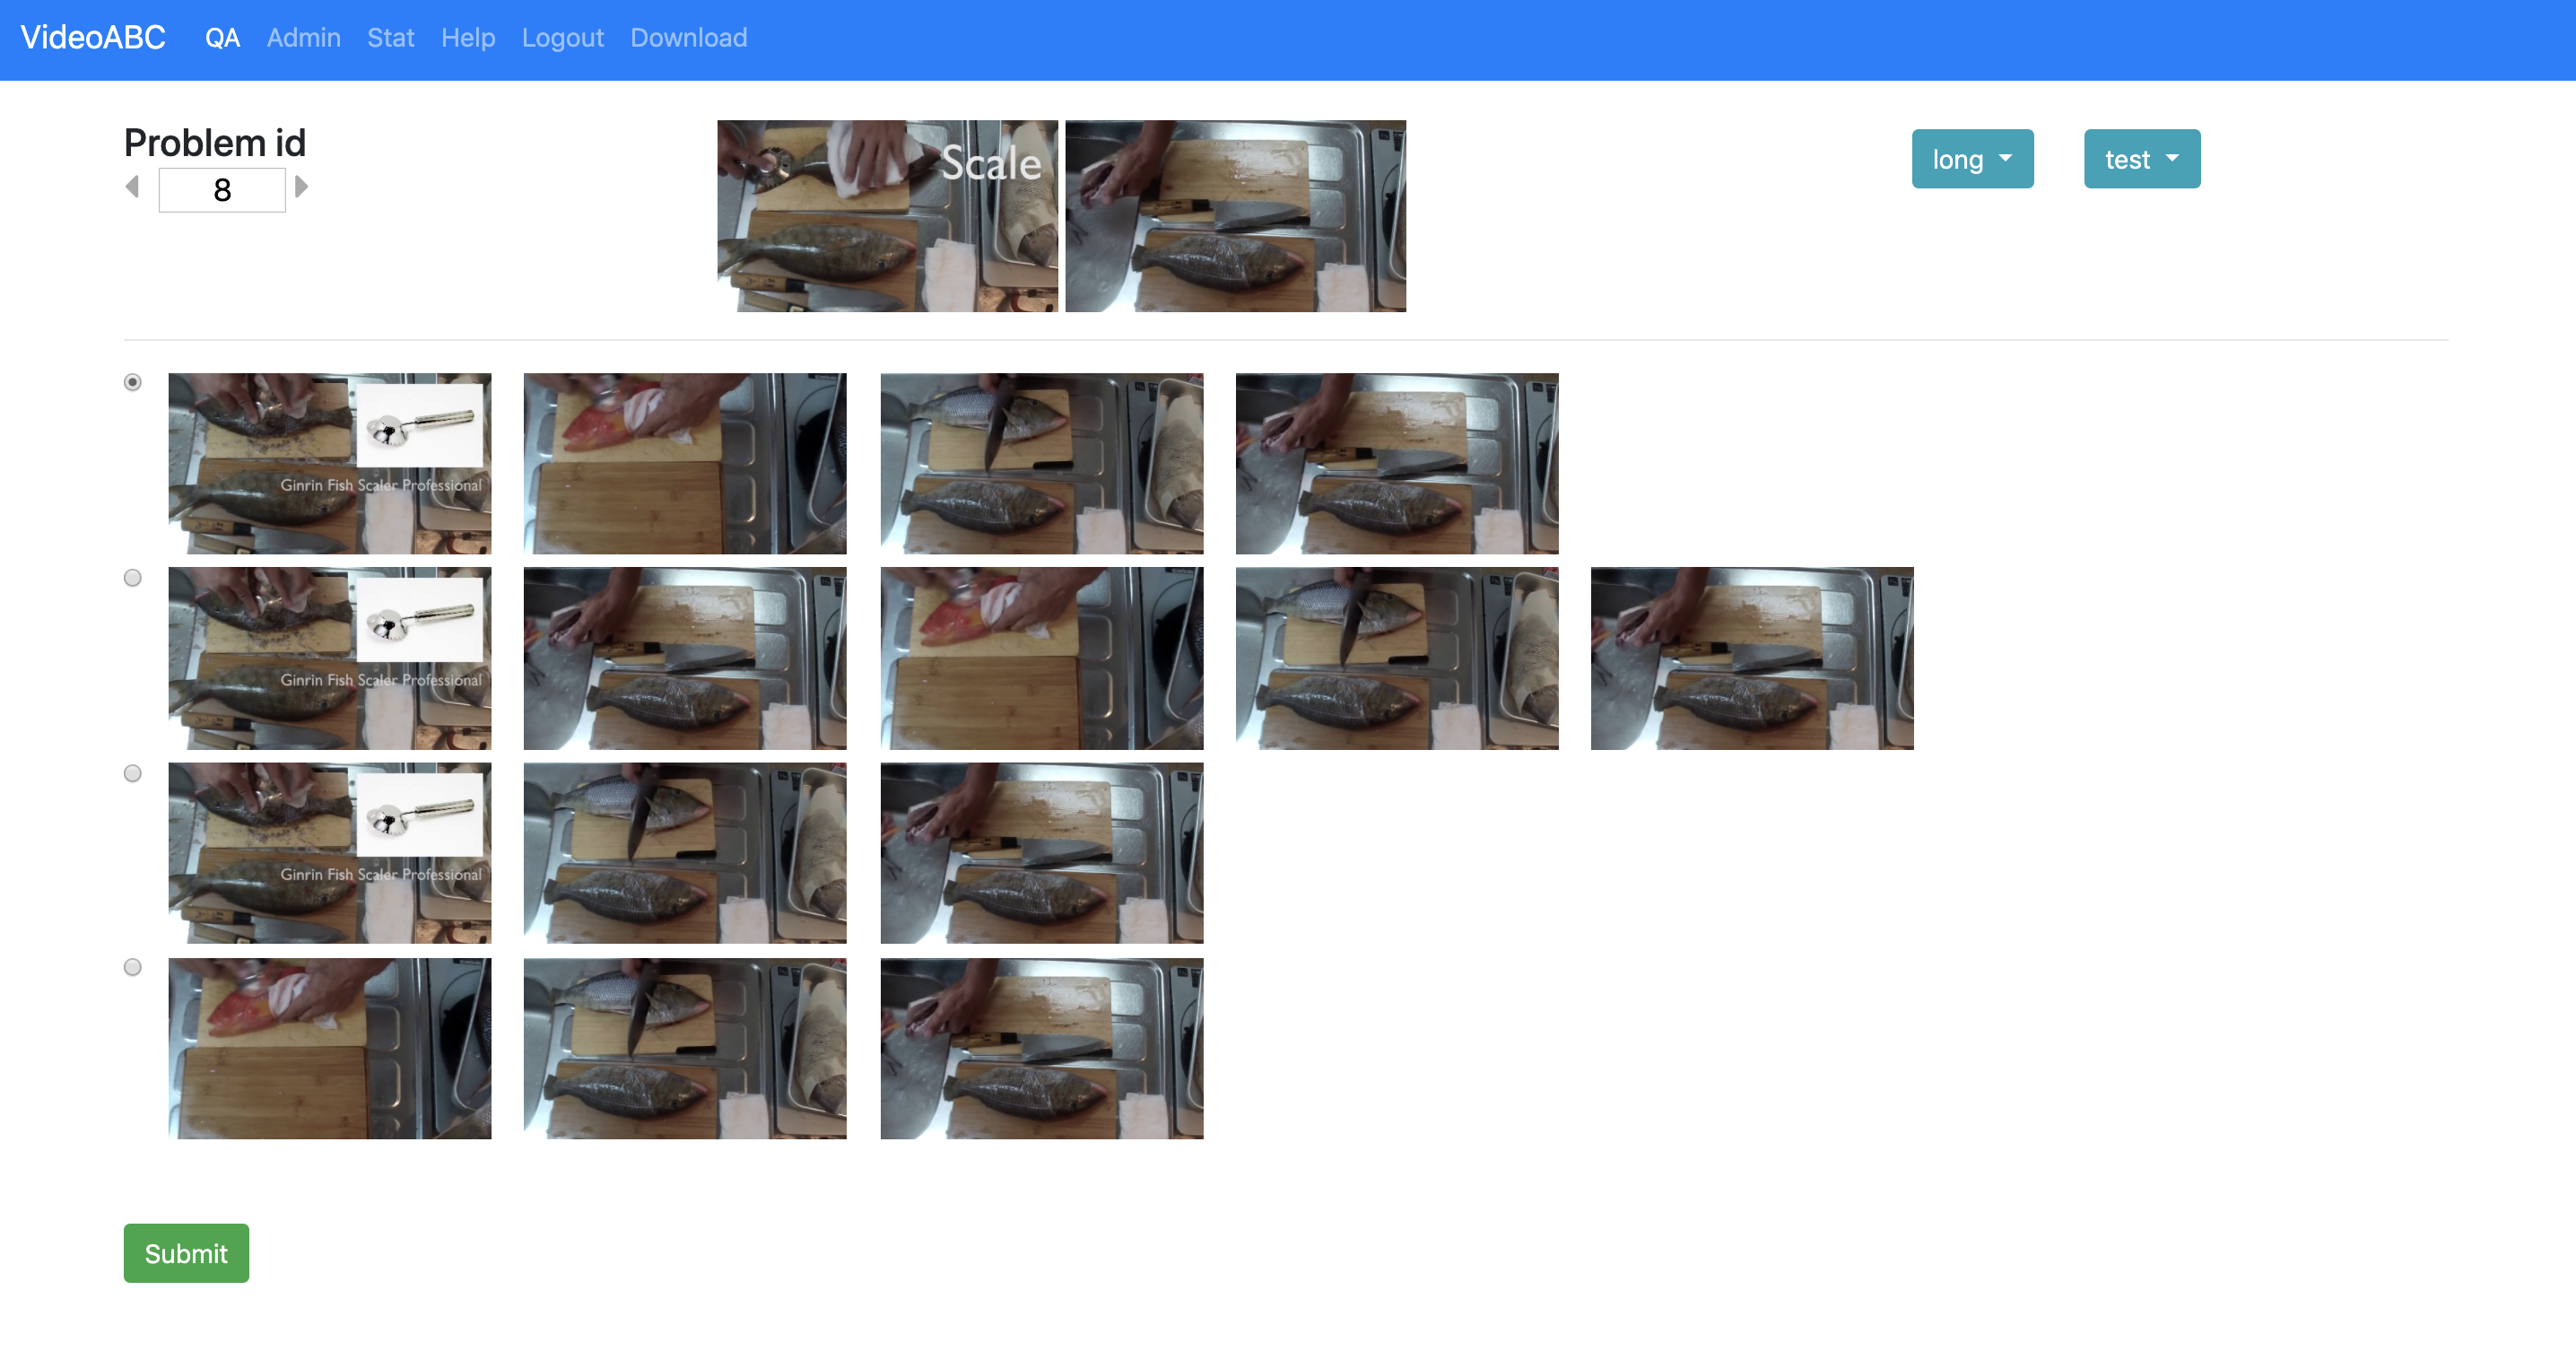
\includegraphics[width=\textwidth]{humantest.png}
    \caption{人类水平测试工具界面}
    \label{fig:humantest}
\end{figure}
测试工具的后端使用Django框架,前端使用Bootstrap框架。与标注工具不同的是,测试工具中需要记录每个测试者的成绩,所以需要设计注册和登录系统。注册和登录系统的界面如图~\ref{fig:sign}~所示。用户在访问标注工具时,必须先完成登录,若没有账号则需要注册一个账号。登录后,用户的信息会保存在cookie中,只要不登出就会始终保持登录状态。Django框架中内置了一套认证系统,包含了各种常见的账号操作,例如登录、登出、修改密码等等,编写代码时只需要完成与各个URL对应的HTML即可,Django 会自动完成与数据库的交互。登录操作则可以通过Django内置的用户表单类来实现。

\begin{figure}[htbp]
    \centering
    \begin{subfigure}{.5\textwidth}
        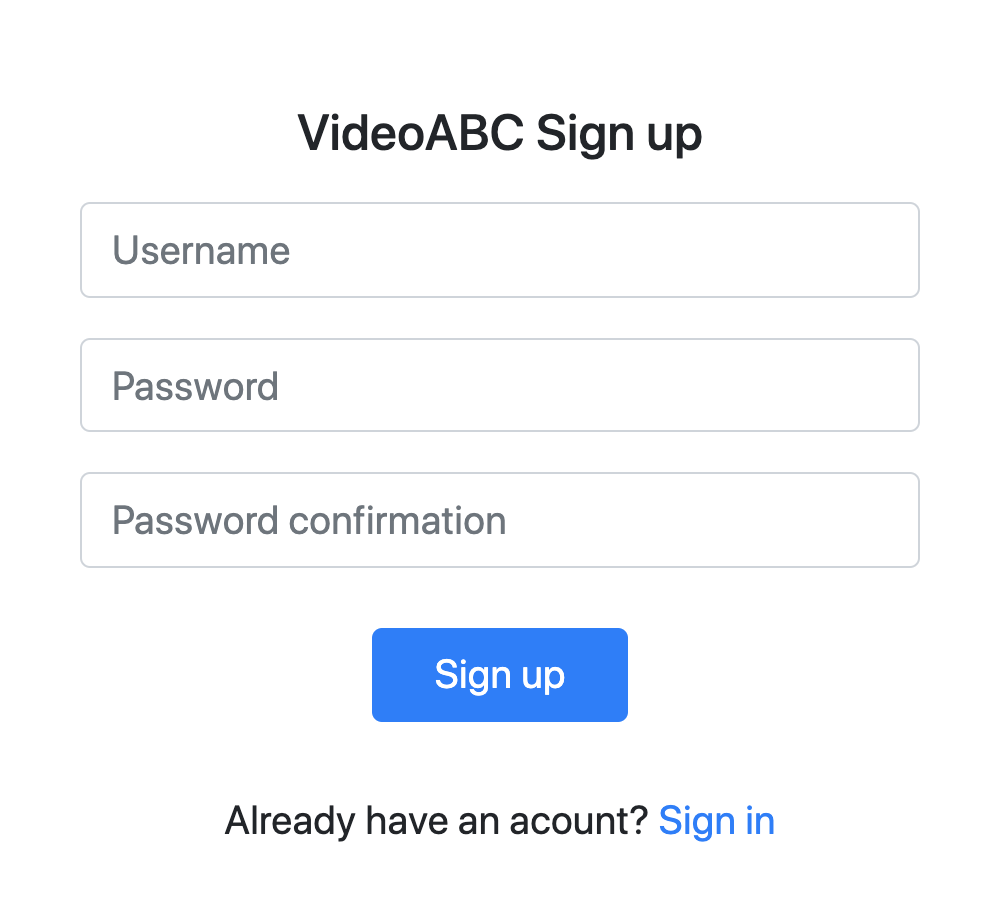
\includegraphics[width=\textwidth{}]{signup.png}
        \caption{注册界面}
    \end{subfigure}%    
    \begin{subfigure}{.5\textwidth}
        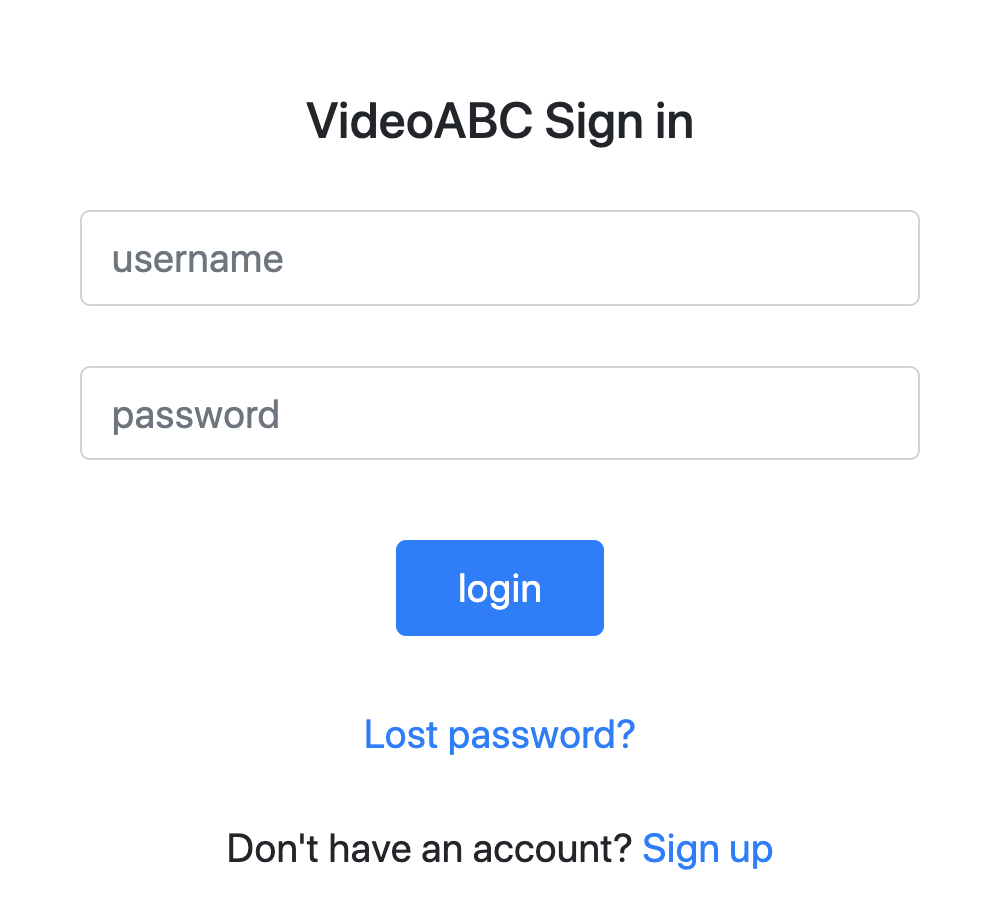
\includegraphics[width=\textwidth{}]{signin.png}
        \caption{登录界面}
    \end{subfigure}%
    \caption{注册和登录界面}
    \label{fig:sign}
\end{figure}

除了注册和登录功能之外,比较重要的部分就是数据结构的设计。测试工具中的一个基本的数据结构是Problem类,每个Problem对象表示一个问题,其主要成员变量如表~\ref{tab:problem}~所示。其中observation和hypothesis中存放的是图片的路径,不同的路径之间用逗号分隔;测试人员回答的答案以序号(0$\sim$3)保存。当测试人员提交答案时,该答案会添加到answers 中,而该用户的用户名会添加到answerers中,且保证顺序一致。答案保存后则从数据库中寻找该用户还没有回答过的问题,来作为该用户的下一个问题,这就保证了测试人员重复回答问题。

\begin{table}[htbp]
    \caption{Problem类主要成员变量}
    \label{tab:problem}
    \begin{tabu}to\textwidth{XXX}\toprule
        变量名称 & 变量类型 & 变量含义\\\midrule
        observation & 字符串 & 观测\\
        hypothesis & 字符串 & 假设\\
        answers & 字符串 & 回答\\
        answerers & 字符串 & 回答者\\
        correct\_answer & 小正整型 & 正确答案\\\bottomrule
    \end{tabu}
\end{table}

为了提高测试速度,测试工具中同样设计了快捷键,如表~\ref{tab:test_shortcut}~所示。同样,测试网站中也提供了帮助页面,便于测试人员明确答题规则。另外,测试网站的统计页面可以实时显示用户的答题准确率。

\begin{table}
    \caption{测试工具快捷键}
    \label{tab:test_shortcut}
    \begin{tabu}to\textwidth{XX}\toprule
        键盘按键 & 功能\\\midrule
        \keys{A}	& 选中选项A\\
        \keys{B}    & 选中选项B\\        
        \keys{C}	& 选中选项C\\
        \keys{D}    & 选中选项D\\
        \keys{Enter} & 提交答案\\\bottomrule
    \end{tabu}
\end{table}
\section{VideoABC上的实验结果}\label{sec:exp:results}

\subsection{实验模型}
为了测试不同模型在VideoABC数据集上的表现,本文测试了多种方法。
\paragraph{随机选择} 从所有的候选答案中随机选择一个,该结果可以用来检验数据集中的选项分布是否均匀。
\paragraph{TSN\cite{wang2016temporal}}TSN是一个简单的2D模型。TSN将视频均匀分割成几个片段,每个片段中抽取一帧,并使用2D卷积神经网络对这些帧提取特征,最后再通过一些运算将这些特征融合(取最大值、均值等等)。

\paragraph{TRN\cite{zhou2018temporal}} TRN是在TSN的基础上为了更好地对时序关系建模而提出的。TRN将TSN中特征合并的操作改成用关系网络(Relation Network)来实现,并通过多级的关系网络在不同的分辨率完成特征的融合。

\paragraph{R3D\cite{tran2018closer}} R3D是一个使用3D残差网络构建的视频理解模型。R3D将经典的2D Resnet 中的卷积换成3D卷积,能够很好地提取时空特征,在许多视频理解的任务中都取得了很好的结果。

\paragraph{R(2+1)D\cite{tran2018closer}} R(2+1)D是在R3D的基础上,将3D卷积分解成了空间上的2D卷积和时间上的1D卷积。在一些任务上,R(2+1)D的表现要比传统的3D卷积更好。

\paragraph{Non-Local Network\cite{wang2018non}} Non-Local Network 是以图像处理中的经典算法 Non-local means 的思路构建的一个模型,该模型能够捕捉时空上间隔较远的位置的关系。Non-local block 可以作为一个模块添加到其他的模型中,例如本文的实验中将该模块添加到R3D和R(2+1)D模型中。

\paragraph{HDR Net} 即本文提出的额多级双重推理网络,详见第~\ref{cha:HDRNet}~章。
\subsection{实现细节}
对于TSN模型,本文使用BNInception的主干网络,与原文的实现\cite{wang2016temporal}保持一致。本文中将每个假设中所有步骤的图片放在一起构成一个视频,将其切分称$K=3$个片段,并从每个片段中抽取1帧,与两个观测一起作为TSN的输入。TSN中的特征融合方法采取了两种方法,即取最大值和取平均值。TRN的实现构建在TSN上,并使用多级融合的结构\cite{zhou2018temporal}。对于R3D和R(2+1)D,本文使用的pytorch官方的实现方式,以ResNet18\cite{he2016deep}为主干网络。本文提出的HDRNet中也使用ResNet18作为主干网络,这就保证了比较的公平性。由于每个假设中的步骤数目不同,实验时需要将所有的选项补零来保证每个选项的长度一致。在训练时 HDR Net的输入除了观测和假设,还包括每个假设的步骤数目,这样在用RNN完成推理过程的时候就可以跳过之前用于补零的步骤。在基于视频的模型中(R3D,R(2+1)D),最后的池化操作仅对有效的步骤长度取平均。对于2D的模型中(TSN,TRN),在加载数据的时候就只对有效步骤分段抽帧即可,不需要补零操作。对于人类水平的测试,本文列出了四位测试人员的平均准确率。

\subsection{实验结果}
表~\ref{tab:results}~展示了上文所述的不同方法的实验结果,以测试集上回答问题的准确率来衡量这些方法的表现。从中可以看到:

\begin{itemize}
    \item 随机选择答案的准确率为25\%,说明了测试集中四个选项的分布比较均匀;
    \item 基于TSN的三种方法中,使用取平均值和取最大值融合的方法表现较差,与随机选择的准确率相差不大。使用关系网络(TRN)虽然有所提升,但准确度仍然很低。这说明基于2D卷积网络再进行特征融合的方法不适合VideoABC数据集;
    \item 基于视频的方法总体上表现较好。其中,R(2+1)D的准确率比R3D要高,说明将3D卷积分解为空间和时间上的卷积的做法有益于提取时空特征。另外,Non-Local模块也能一定程度上提升分类的准确率;
    \item 本文提出的HDR Net 在所有的模型上表现最好,超出其他最好的模型将近9个百分点。这是因为HDR Net专门为视频溯因常识推理任务而设计,能够成功地对步骤内和步骤间的时序关系建模;
    \item 人类的表现为92.4\%,远超其他所有的模型。这说明人类确实可以利用已有的常识取得比模型更好的表现。
\end{itemize}

\begin{table}[htbp]
\caption{不同模型的在VideoABC上的准确率}   
\label{tab:results}
\begin{tabu}to\textwidth{XX}\\
\toprule
   模型/方法 & 准确率 (\%) \\
    \midrule
    Random & 25.0 \\
    \midrule
    TSN-\texttt{average}~\cite{wang2016temporal} & 24.9\\
    TSN-\texttt{max}~\cite{wang2016temporal} & 27.6\\
	TRN~\cite{zhou2018temporal} & 37.3\\
	\midrule
	R3D~\cite{R3D} & 74.2\\
	R(2+1)D~\cite{R3D} & 74.5\\
	R3D + Non-Local~\cite{wang2017non} & 74.3\\
	R(2+1)D + Non-Local ~\cite{wang2017non} & 76.0\\
	\midrule
	\textbf{HDRNet} & \textbf{85.2}\\
	\midrule
	Human & 92.4\\\bottomrule
    \end{tabu}
\end{table}

\section{消融实验}\label{sec:exp:ablation}
\subsection{步骤数目变化的影响}
在第~\ref{cha:VideoABC}~章中,本文介绍过VideoABC数据集的构建方式,在步骤切分和筛选的步骤中曾指定了最小步骤数$m=2$和最大步骤数$M=6$,本节中将探究不同步骤数对实验结果的影响。表~\ref{tab:VideoABC_steps}~列举了不同的配置以及命名。在这些配置中,$M$从1到6变化。由于需要保证$m\le M$,当$M=1$时,$m=1$。此时第~\ref{cha:VideoABC}~章中提到的错误选项类型中将不存在交换和删除,且正确选项中只包含一个步骤,推理时长较短,所以将其命名为short,意为短时推理(Short Time Reasoning, STR)。另外的几种配置则对应长时推理(Long Time Reasoning, LTR),对应着long2到long6的命名,其中的数字表示正确选项中的最大步骤数目$M$。需要注意的是,在LTR的任务中,所有选项的最长步骤应该为$M+1$(考虑到“插入”的错误类型)。与之前生成数据集的方式一样,表~\ref{tab:VideoABC_steps}~中不同配置的数据集也是经过难分选项挖掘的。

\begin{table}[htbp]
    \caption{不同步骤数目的VideoABC数据集}
    \label{tab:VideoABC_steps}
    \begin{tabu}to\textwidth{XXX}\toprule
        最短步骤数$m$ & 最长步骤数$M$ & 名称\\\midrule
        1 & 1 & short\\
        2 & 2 & long2\\
        2 & 3 & long3\\
        2 & 4 & long4\\
        2 & 5 & long5\\
        2 & 6 & long6\\\bottomrule
    \end{tabu}
\end{table}

\begin{table}
    \caption{不同步骤数目的实验结果}
    \begin{tabu}to \textwidth{l*{6}{X[c]}}\\
        \toprule
            方法 & $M=1$ & $M=2$ & $M=3$ & $M=4$ & $M=5$ & $M=6$\\
            \midrule
        Random & 25.0 & 25.0 & 25.0 & 25.0 & 25.0 & 25.0\\
         \midrule
        TSN-\texttt{average} & 30.2 & 18.3 & 15.3 & 17.1 & 14.6 & 16.4 \\
        TSN-\texttt{max} & 24.1 & 26.4 & 29.3 & 27.6 & 26.9 & 28.6 \\
         \midrule
        R3D & 84.7 & 85.5 & 79.1 & 74.4 & 73.9 & 73.1 \\
        R(2+1)D & 86.9 & 86.8 & 81.6 & 74.4 & 74.4 & 74.5 \\
         \bottomrule
        \end{tabu}
\end{table}

\subsection{难分样本挖掘的作用}
\subsection{网络结构和大小的影响}
\section{概率模型检验}\label{sec:exp:prob}
VideoABC数据集的一个特点在于,模型必须对两个观测有全面的理解才能选出正确的答案,而不能只从选项中通过一些捷径判断。为了验证观测信息的重要性,本文利用第~\ref{sec:abductive}~节中介绍过的概率模型来对VideoABC数据集进行实验。本节中的实验所用模型

% !TeX root = ../main.tex

\chapter{总结}\label{cha:close}
为了解决当前视觉推理任务中存在的一些问题,本文提出了一个新的视觉推理任务:视频溯因常识推理,在该任务中,模型需要根据表示开始状态和结束状态的两个观测$O_1$和$O_2$从候选假设集合$\{H_i\}$中选出正确答案,其中每个假设由一系列基本步骤构成,而每个步骤以一个视频片段的形式呈现。

根绝视频溯因常识推理的任务定义,本文构建了VideoABC数据集。该数据集以教程类数据集COIN\cite{tang2019coin}为基础,通过二次标注保证了推理过程的连续性,并通过预定义的四种错误类型构建出候选假设集合,最后使用难分样本挖掘的方式来去除过于简单的假设,从而提升VideoABC数据集的难度。最后的VideoABC数据集中共包含13,522个问题,最大的推理时长高达731s,这对模型完成长时间推理的能力来说是一个很大的挑战。

实验发现,大部分在视频理解上表现较好的模型都不能在VideoABC数据集上取得很好的效果。为此,本文针对视频溯因常识推理任务设计了一个新的模型:多级双重推理网络(HDR Net)。该网络以ResNet18\cite{he2016deep}为基础,在每个空间的池化层后面都加入一个步骤内推理模块和步骤间推理模块,从而能够有效地挖掘步骤内和步骤间的时序关系。步骤内和步骤间推理模块都使用双向RNN的结构,并使用残差连接的方式来更新特征。实验表明,HDR Net在VideoABC上的表现远超其他的模型。

此外,为了检验人类在VideoABC数据集上的表现,本文开发了在线测试工具,发现人类的表现比当前现有的模型(包括HDR Net)都要高,这表明人类基于已有的常识和推理能力能够很好地胜任视频溯因常识推理任务,也说明了在VideoABC数据集上模型还有很大的进步空间。


% 其它部分
\backmatter

%% 本科生要求的几个索引。
\listoffigures    % 插图索引
\listoftables     % 表格索引
\listofequations  % 公式索引

% 参考文献
% \bibliographystyle{thuthesis-numeric}      % 顺序编码制
% \bibliographystyle{thuthesis-author-year}  % 著者-出版年制
\bibliographystyle{thuthesis-bachelor}     % 本科生参考文献的著录格式
\bibliography{ref/refs,ref/misc}

% 致谢
\input{data/acknowledgements}

% 声明
\statement

% 附录
\appendix
% \input{data/appendix-survey}       % 本科生:外文资料的调研阅读报告
% \input{data/appendix-translation}  % 本科生:外文资料的书面翻译
\input{data/appendix}

% 个人简历
\input{data/resume}

% 本科生的综合论文训练记录表
% \includepdf[pages=-]{scan-record.pdf}

\end{document}
